\section{Results} 
\label{sec:results}

\todo{todo results}

\begin{figure}[H]
  \centering
  \begin{subfigure}{0.5\textwidth}
    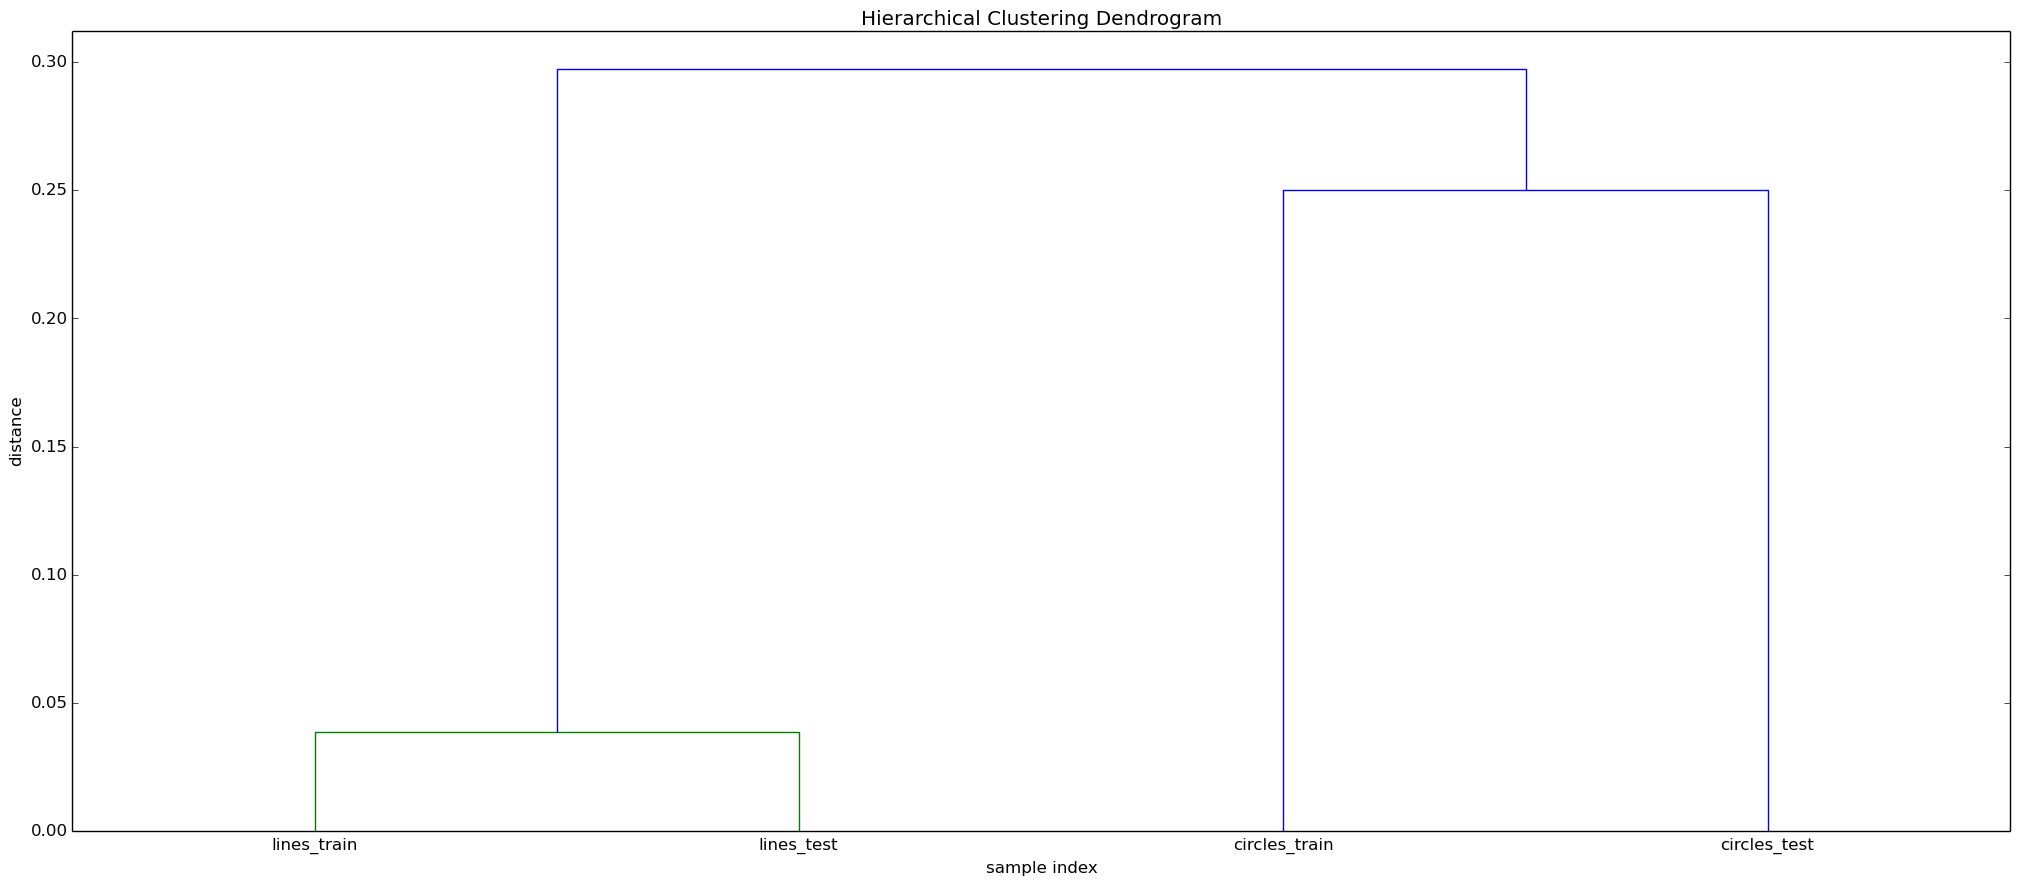
\includegraphics[width=\textwidth]{{img/sample}}
    \caption{Subfigure 2(A)}
    \label{fig:2a}
  \end{subfigure}~
  \begin{subfigure}{0.5\textwidth}
    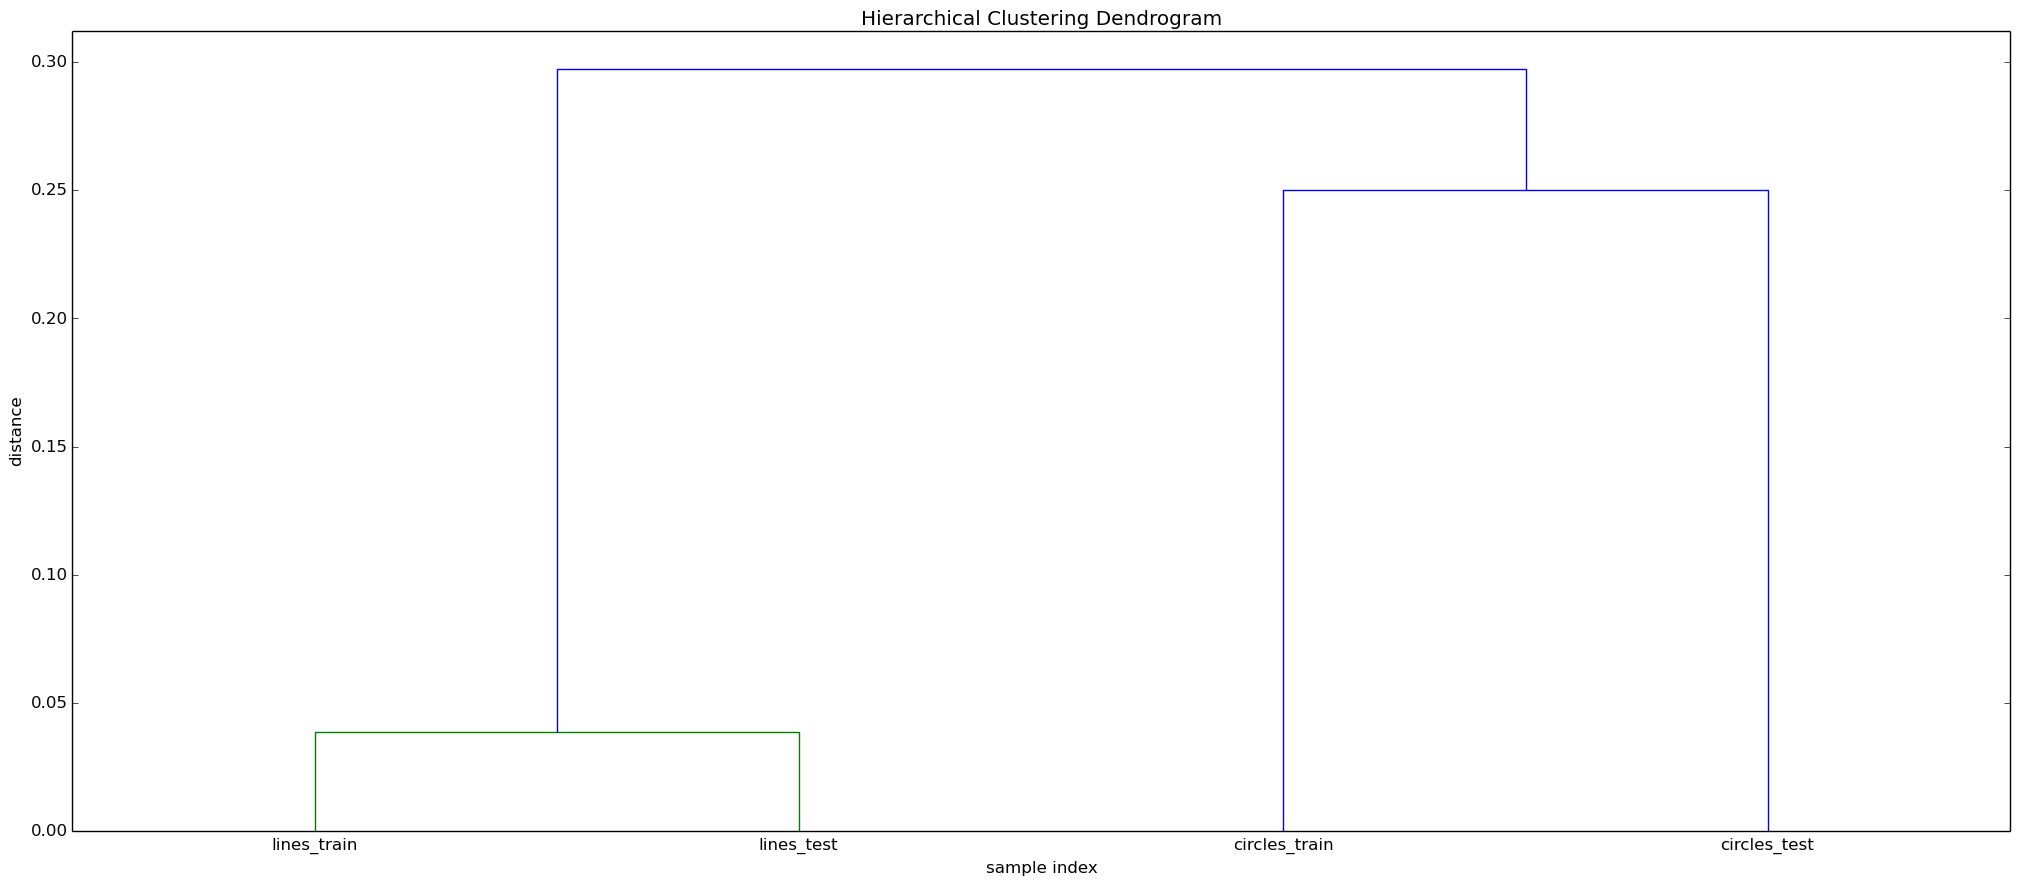
\includegraphics[width=\textwidth]{{img/sample}}
    \caption{Subfigure 2(B)}
    \label{fig:2b}
  \end{subfigure}
  \begin{subfigure}{0.5\textwidth}
    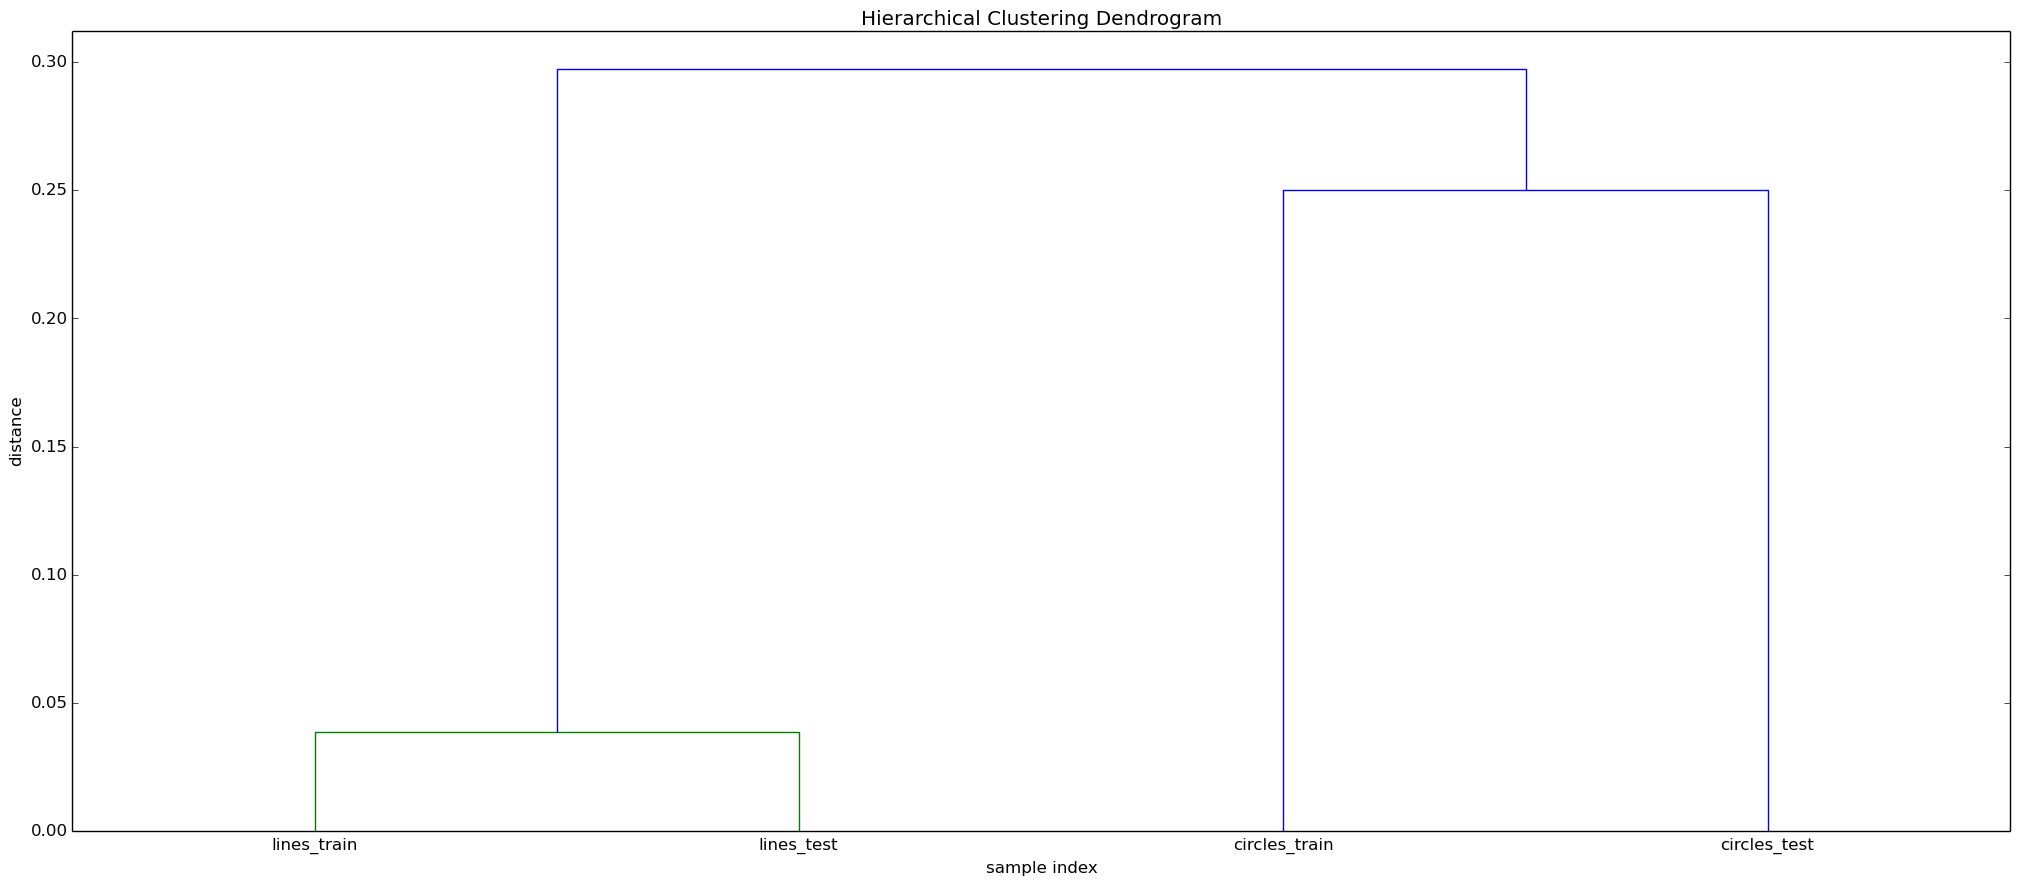
\includegraphics[width=\textwidth]{{img/sample}}
    \caption{Subfigure 2(C)}
    \label{fig:2c}
  \end{subfigure}~
  \begin{subfigure}{0.5\textwidth}
    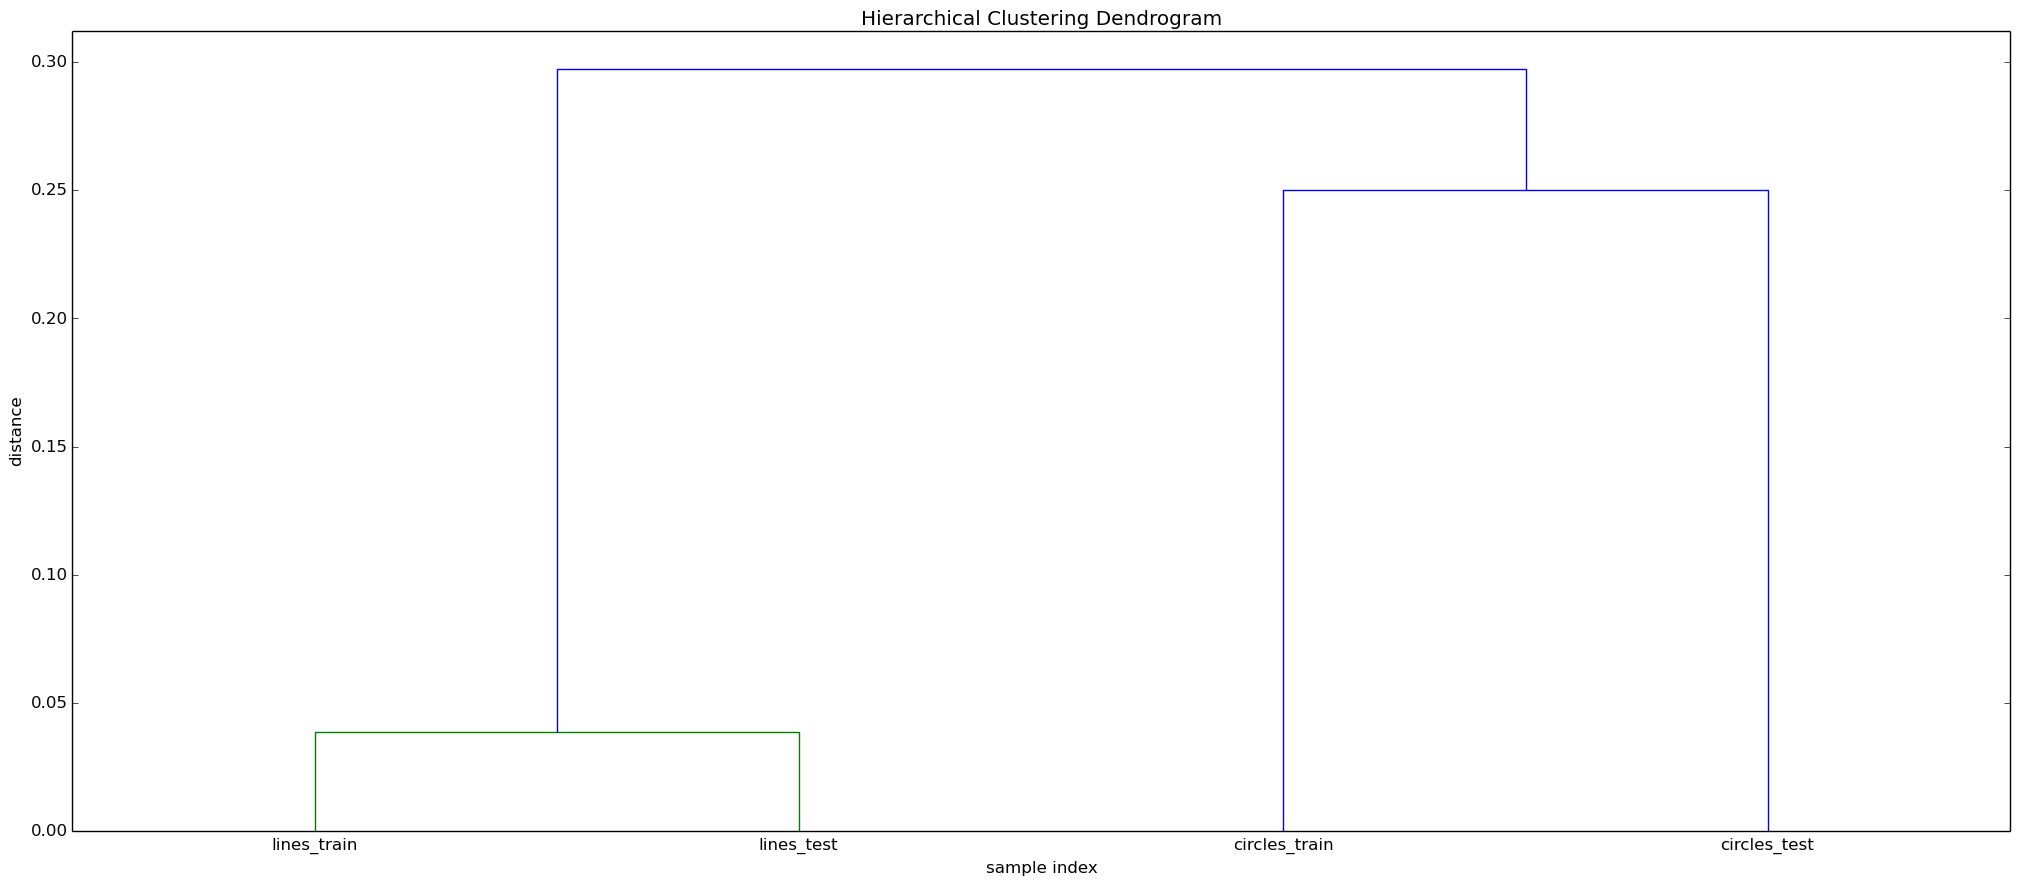
\includegraphics[width=\textwidth]{{img/sample}}
    \caption{Subfigure 2(D)}
    \label{fig:2d}
  \end{subfigure}
  \caption{Four Subfigures}
  \label{fig:fig_2}
\end{figure}

To visualize persistances of homology groups we used the bar code diagrams and persistance diagrams. The bar code diagram for a certain homology group $H$ is a two dimensional plot that shows us the life spans of all the homology classes. For each homology class $\gamma$ we plot a line segment that starts in point $(i_{\gamma}, y_{\gamma})$ and ends in point $(j_{\gamma}, y_{\gamma})$, where $i_{\gamma}$ and $j_{\gamma}$ are life and death of $\gamma$ and $y_{\gamma}$ is a unique number that represents $\gamma$ on the $y$ axis of the plot.\\
\\
Persistance diagrams show the same information in the form of a scatter plot. For each $\gamma$, $pers(\gamma) = [i_{\gamma}, j_{\gamma}]$ in some homology group we just plot the point $(i_{\gamma}, j_{\gamma}$.\\
\\
Here are the barcode diagrams and persistance diagrams obtained for each of the three domains abstracts, sports and reviews. To generate this specific plots we used all the feature functions described in the preperation of data section plus the tf-idf method for the first $50$ most common words. We also used the maximal filtration, meaning filtration (in particulat parameter $r$) was not split to some predetermined number of intervals but just left as is. We were looking at the constructions of cech complexes.

%***********%
% abstracts %
%***********%

\begin{figure}[H]
  \centering
  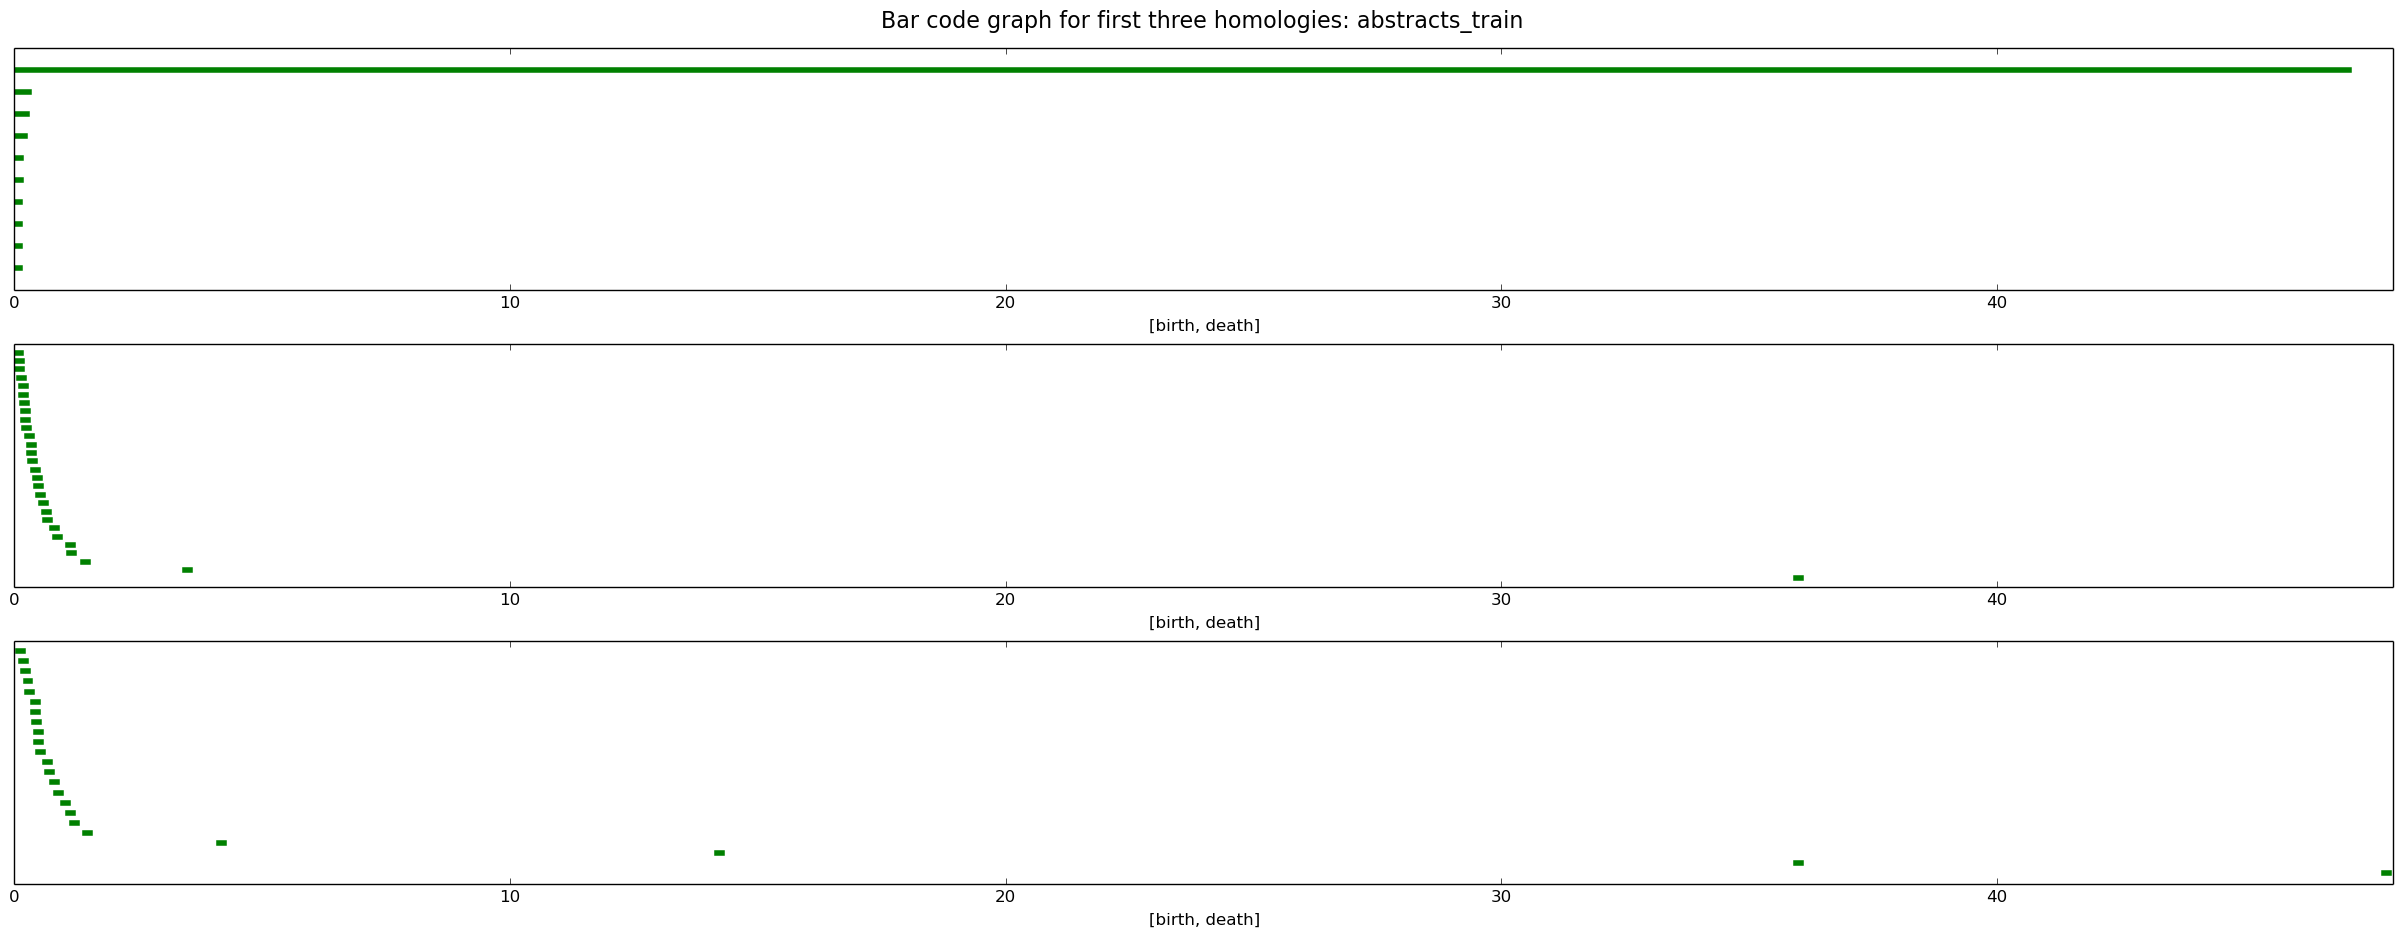
\includegraphics[width=\textwidth]{{img/bar_code_diagram_abstracts_train.png}}
  \caption{Bar codes for abstracts\_train}
  \label{fig:a_1}
\end{figure}
    
\begin{figure}[H]
  \centering
  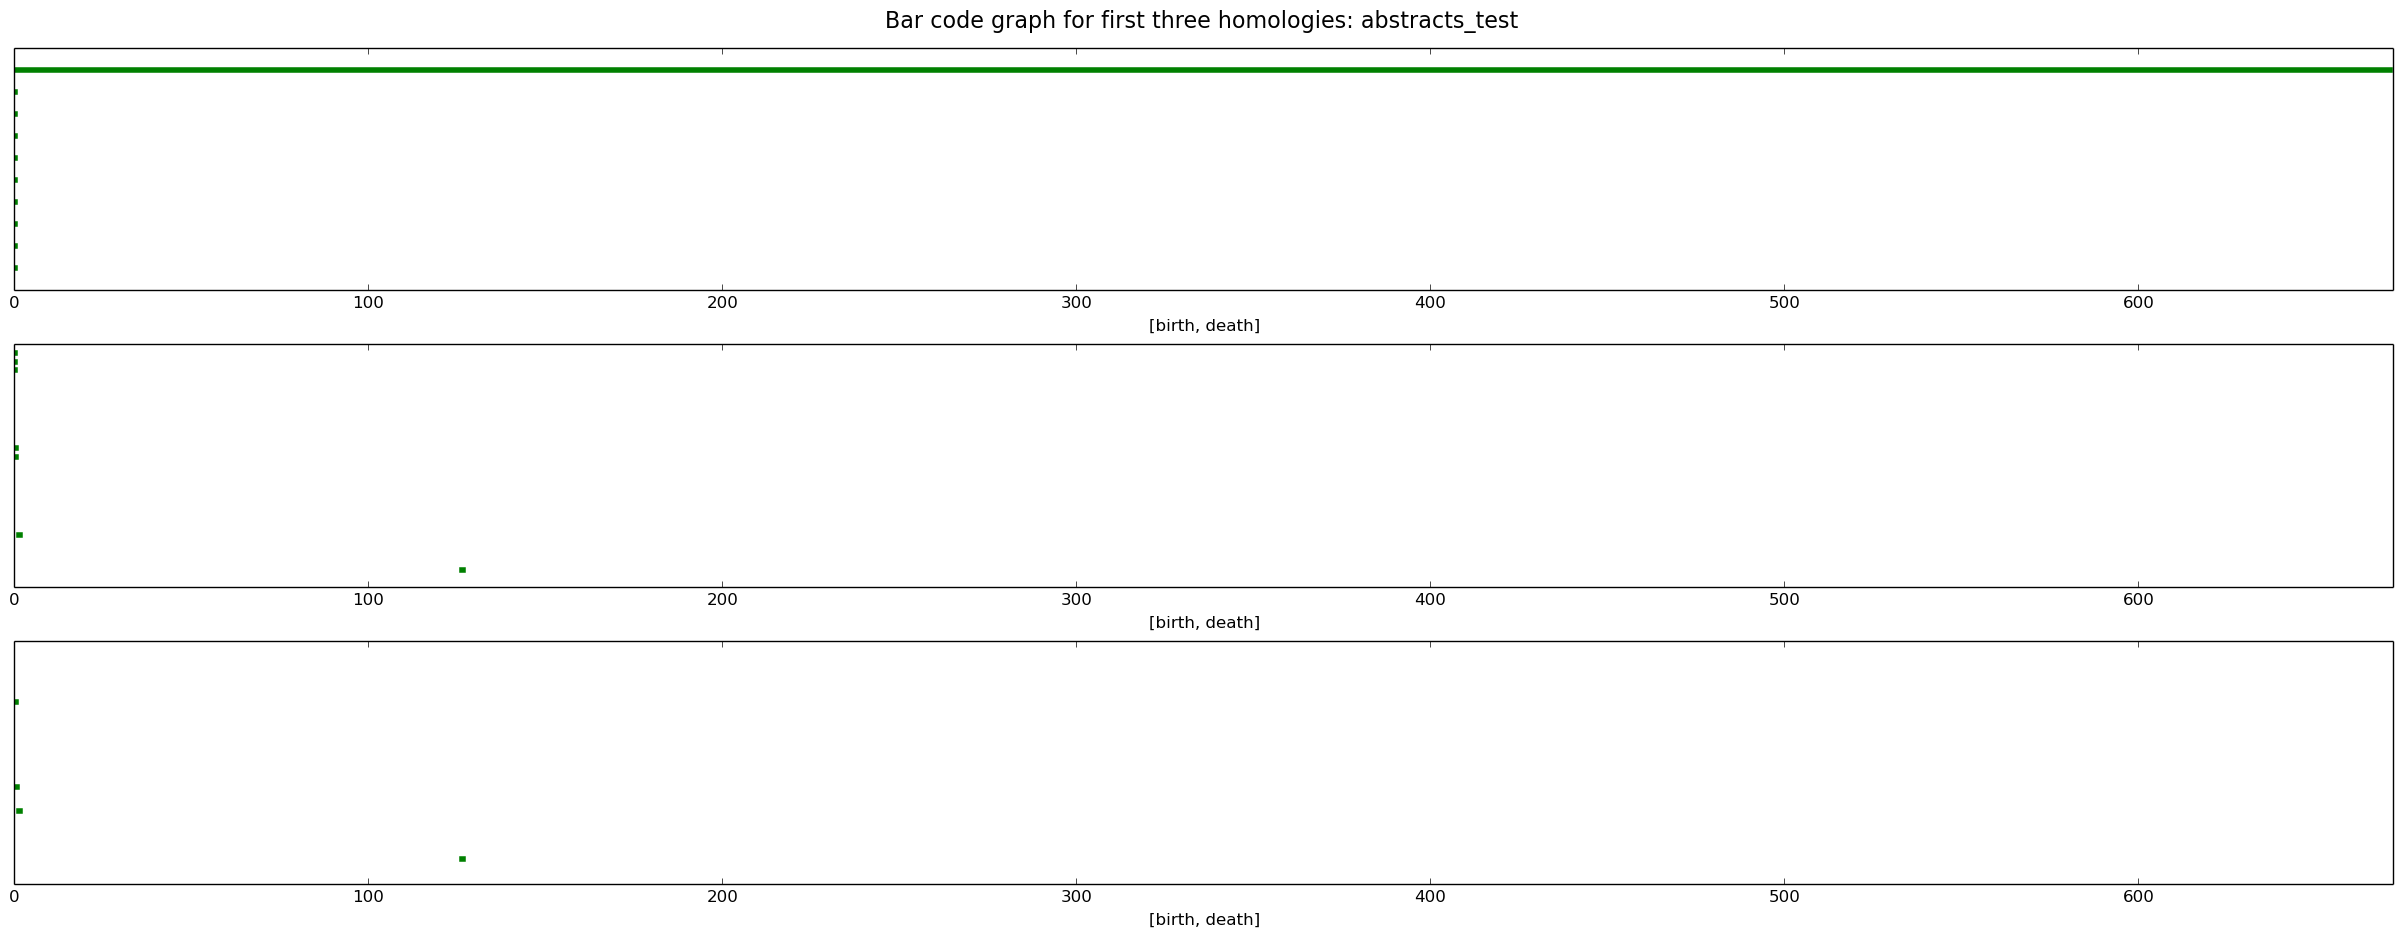
\includegraphics[width=\textwidth]{{img/bar_code_diagram_abstracts_test.png}}
  \caption{Bar codes for abstracts\_test}
  \label{fig:a_2}
\end{figure}

\begin{figure}[H]
  \centering
  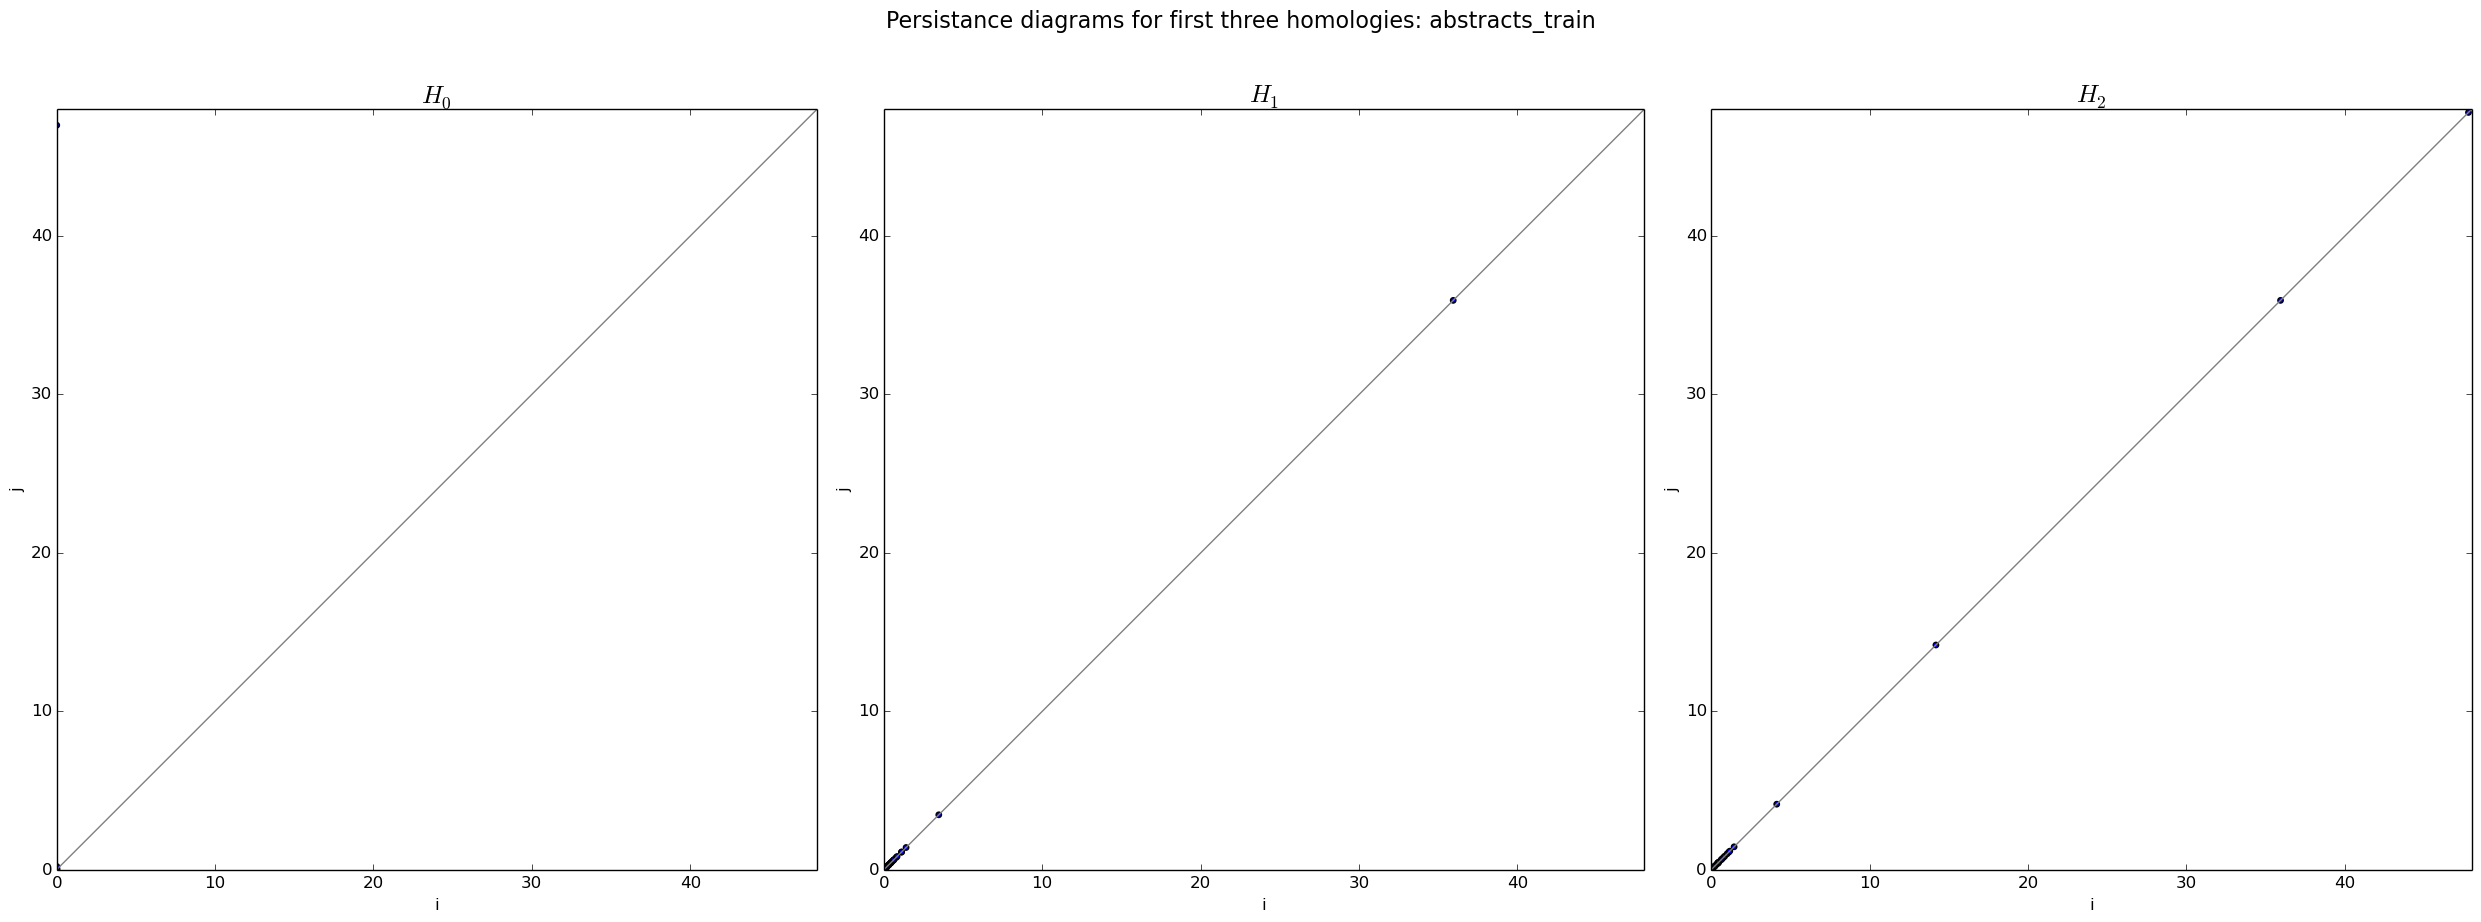
\includegraphics[width=\textwidth]{{img/pers_diagram_abstracts_train.png}}
  \caption{Persistance diagrams for abstracts\_train}
  \label{fig:a_3}
\end{figure}

\begin{figure}[H]
  \centering
  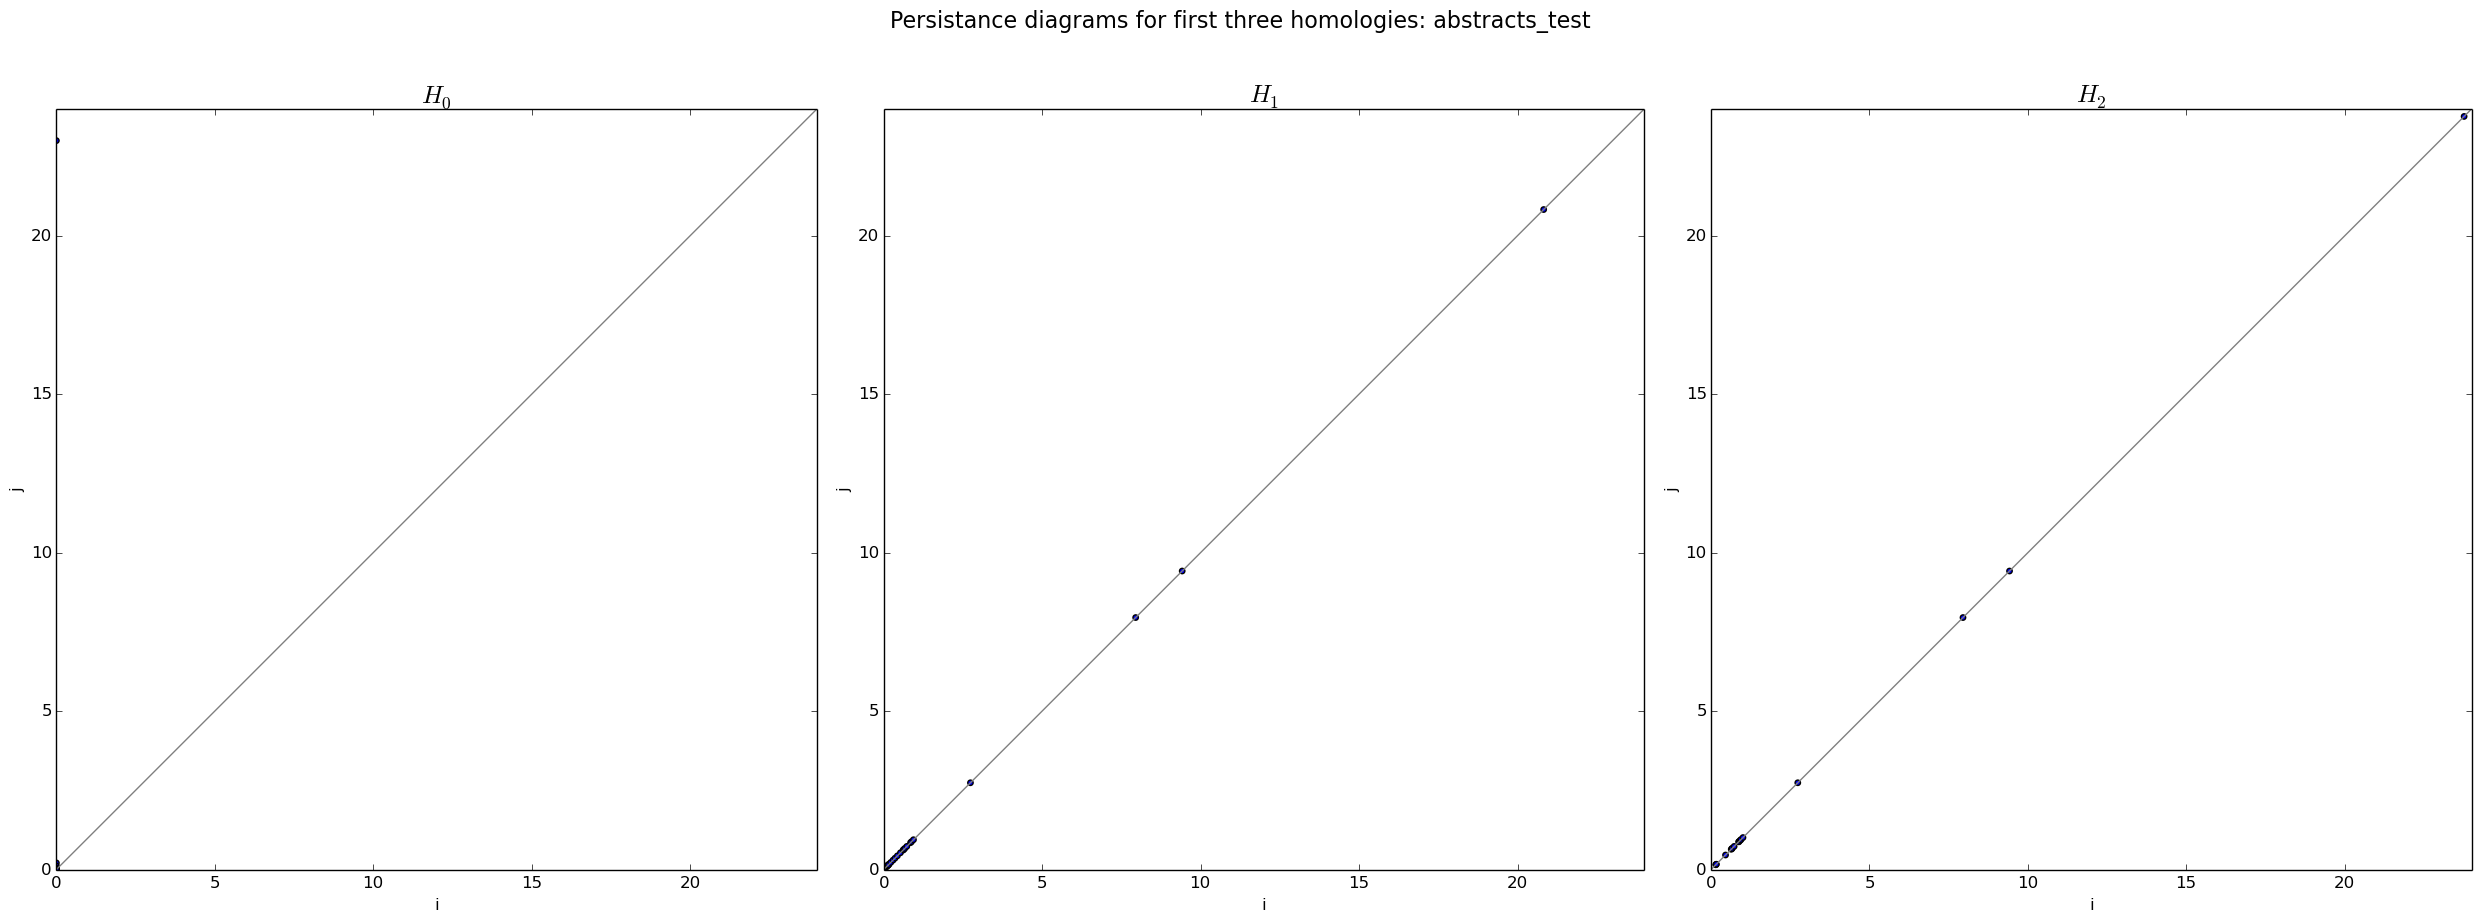
\includegraphics[width=\textwidth]{{img/pers_diagram_abstracts_test.png}}
  \caption{Persistance diagrams for abstracts\_test}
  \label{fig:a_4}
\end{figure}

%********%
% sports %
%********%

\begin{figure}[H]
  \centering
  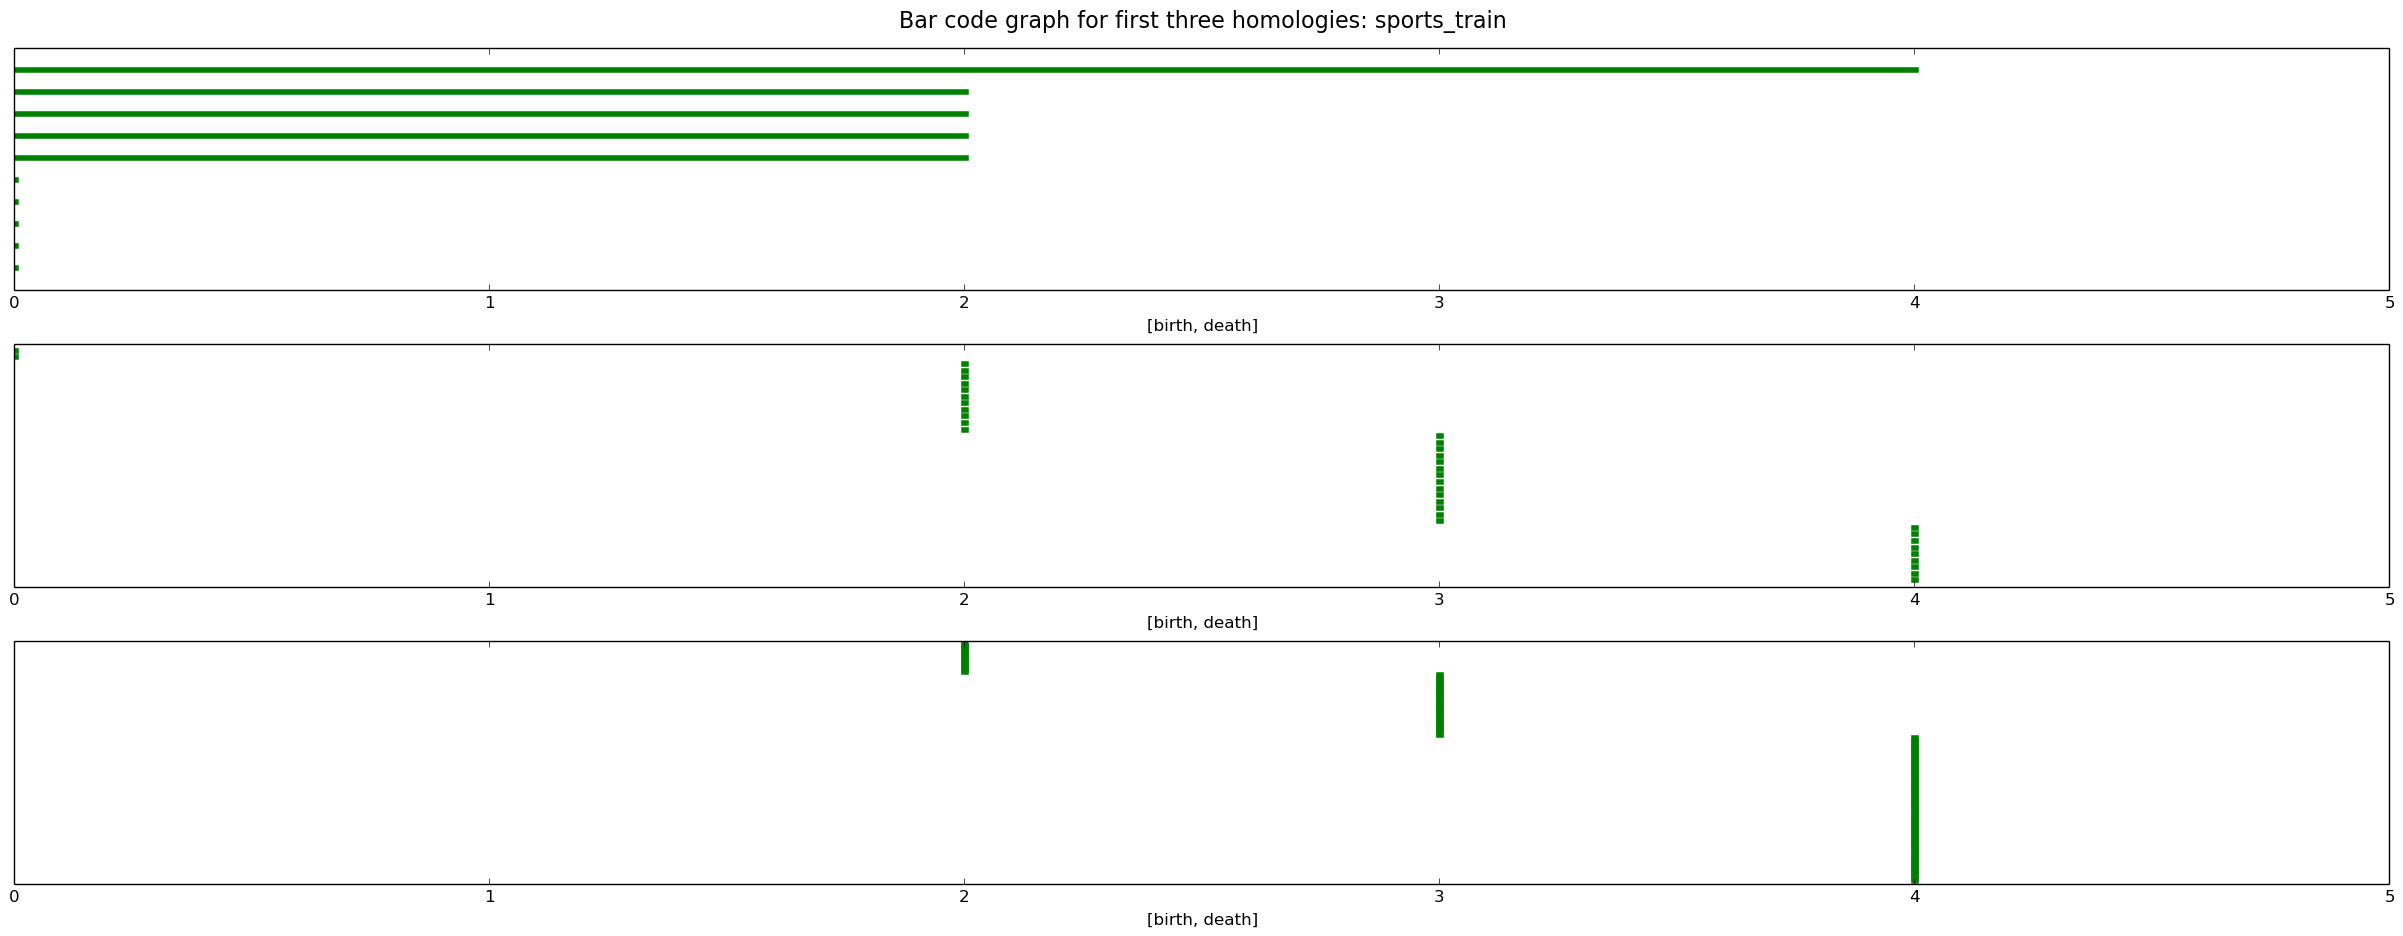
\includegraphics[width=\textwidth]{{img/bar_code_diagram_sports_train.png}}
  \caption{Bar codes for sports\_train}
  \label{fig:s_1}
\end{figure}
    
\begin{figure}[H]
  \centering
  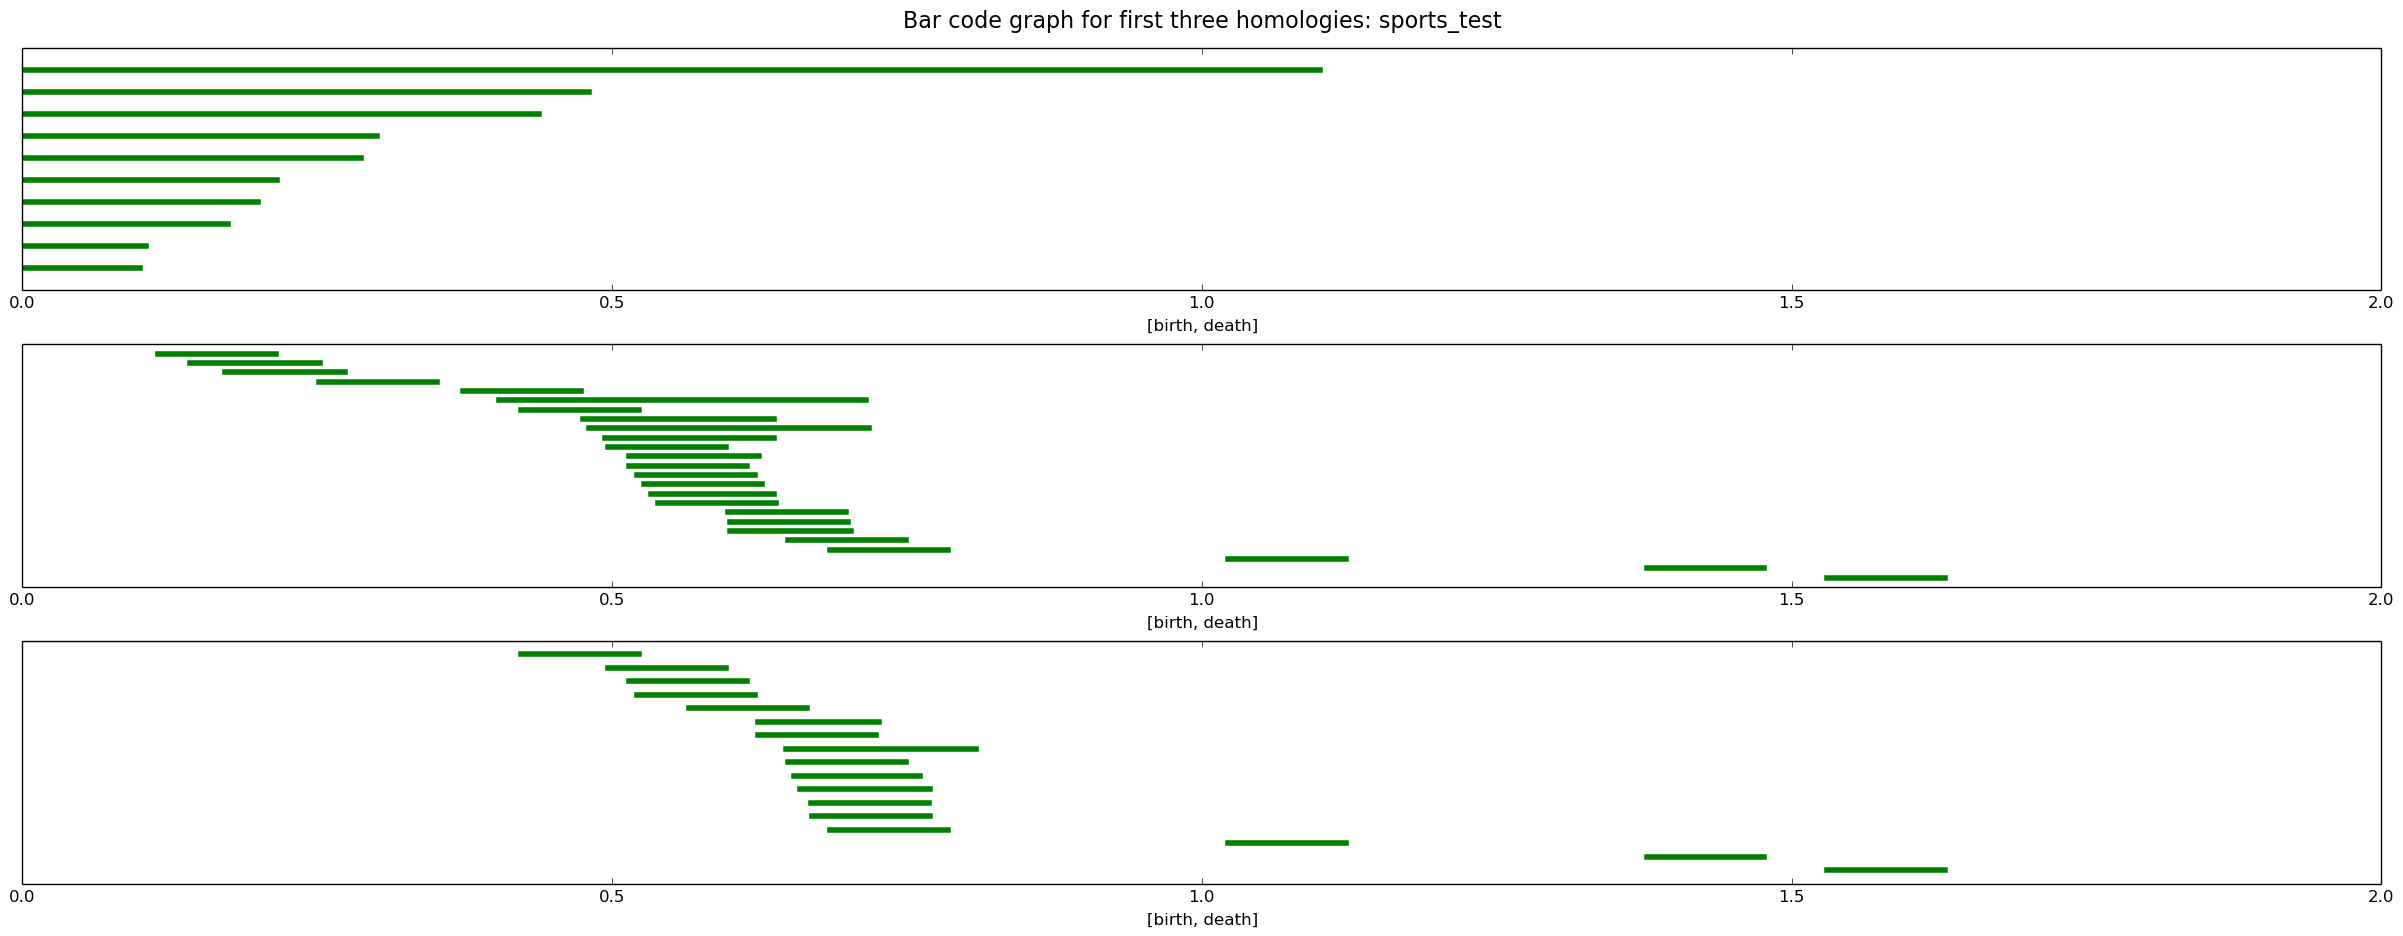
\includegraphics[width=\textwidth]{{img/bar_code_diagram_sports_test.png}}
  \caption{Bar codes for sports\_test}
  \label{fig:s_2}
\end{figure}

\begin{figure}[H]
  \centering
  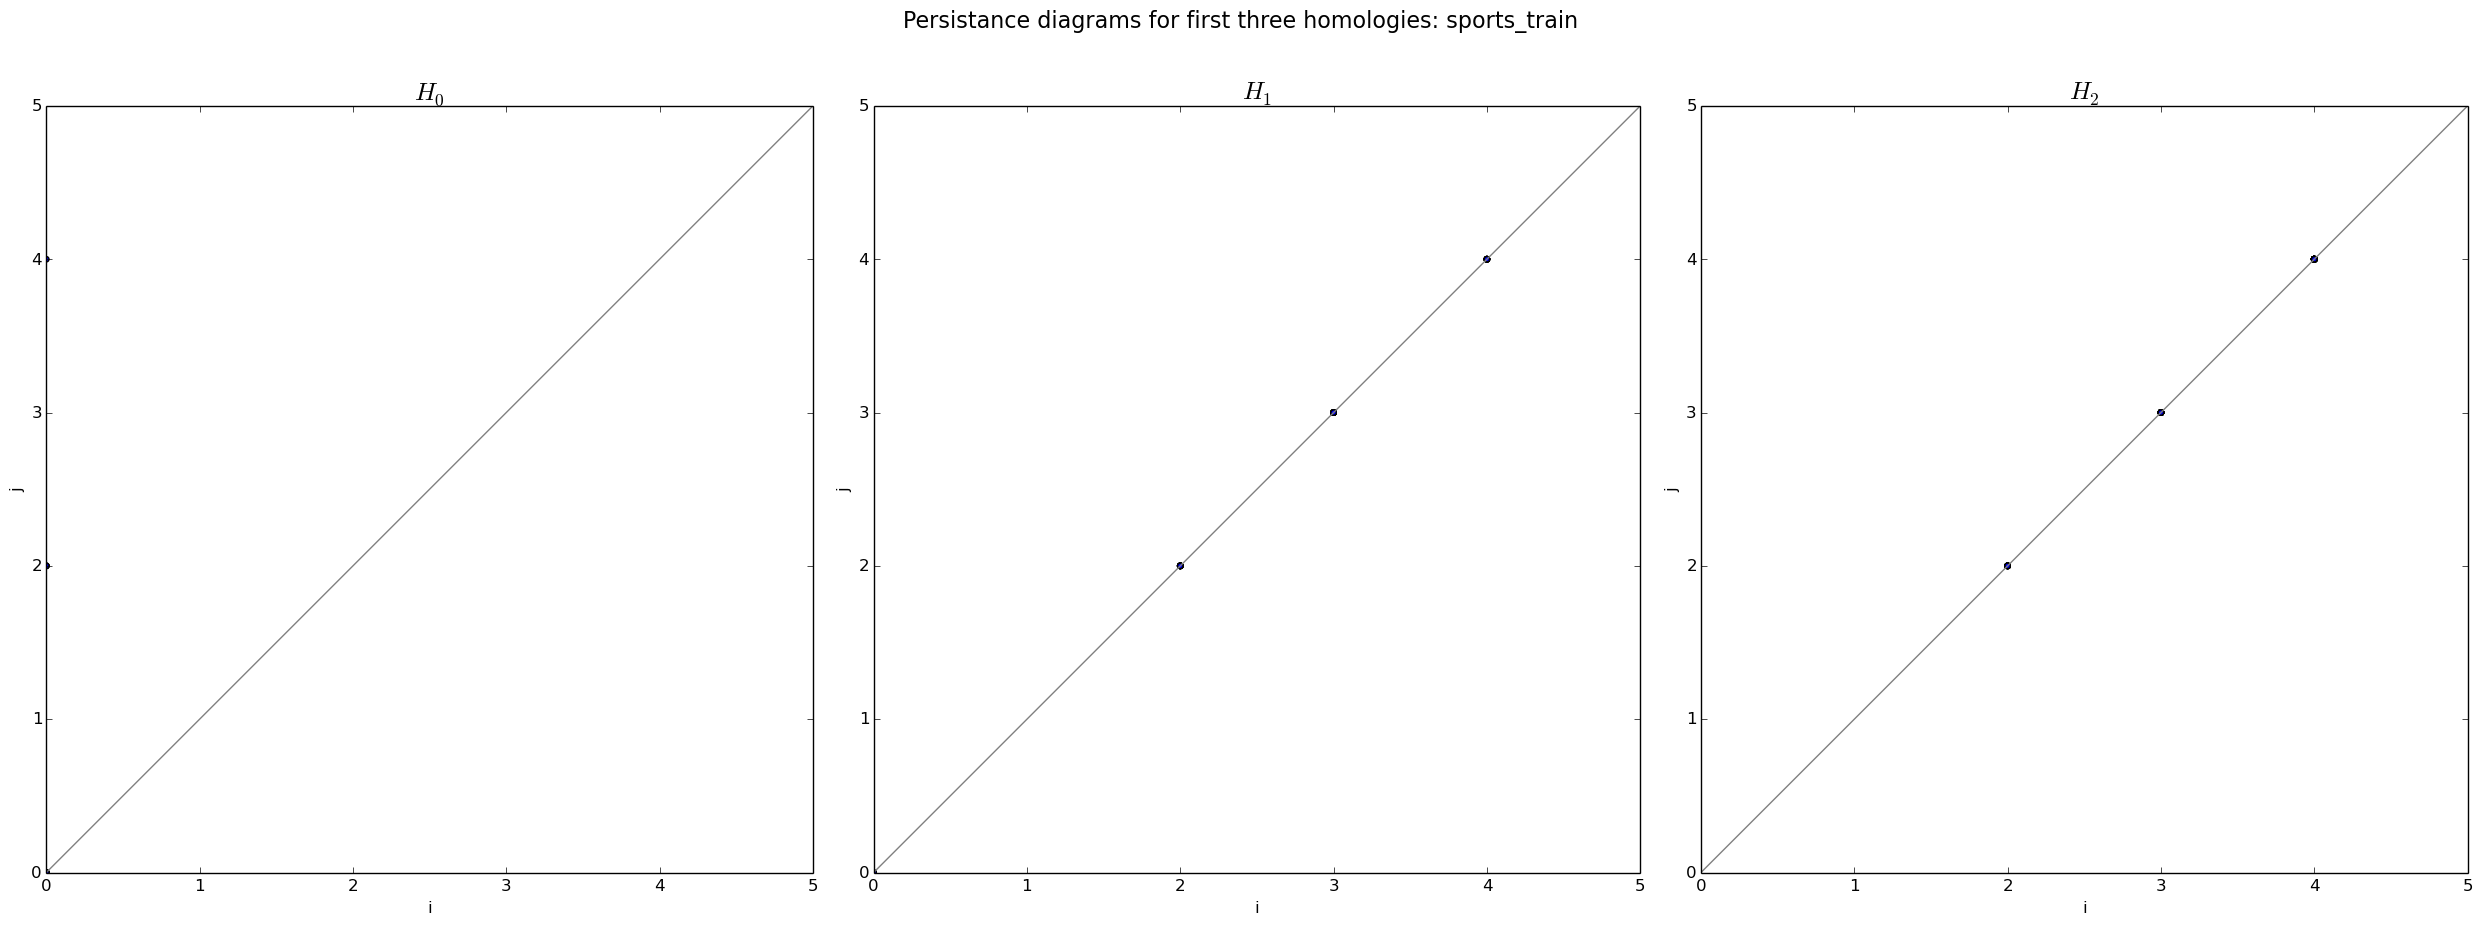
\includegraphics[width=\textwidth]{{img/pers_diagram_sports_train.png}}
  \caption{Persistance diagrams for sports\_train}
  \label{fig:s_3}
\end{figure}

\begin{figure}[H]
  \centering
  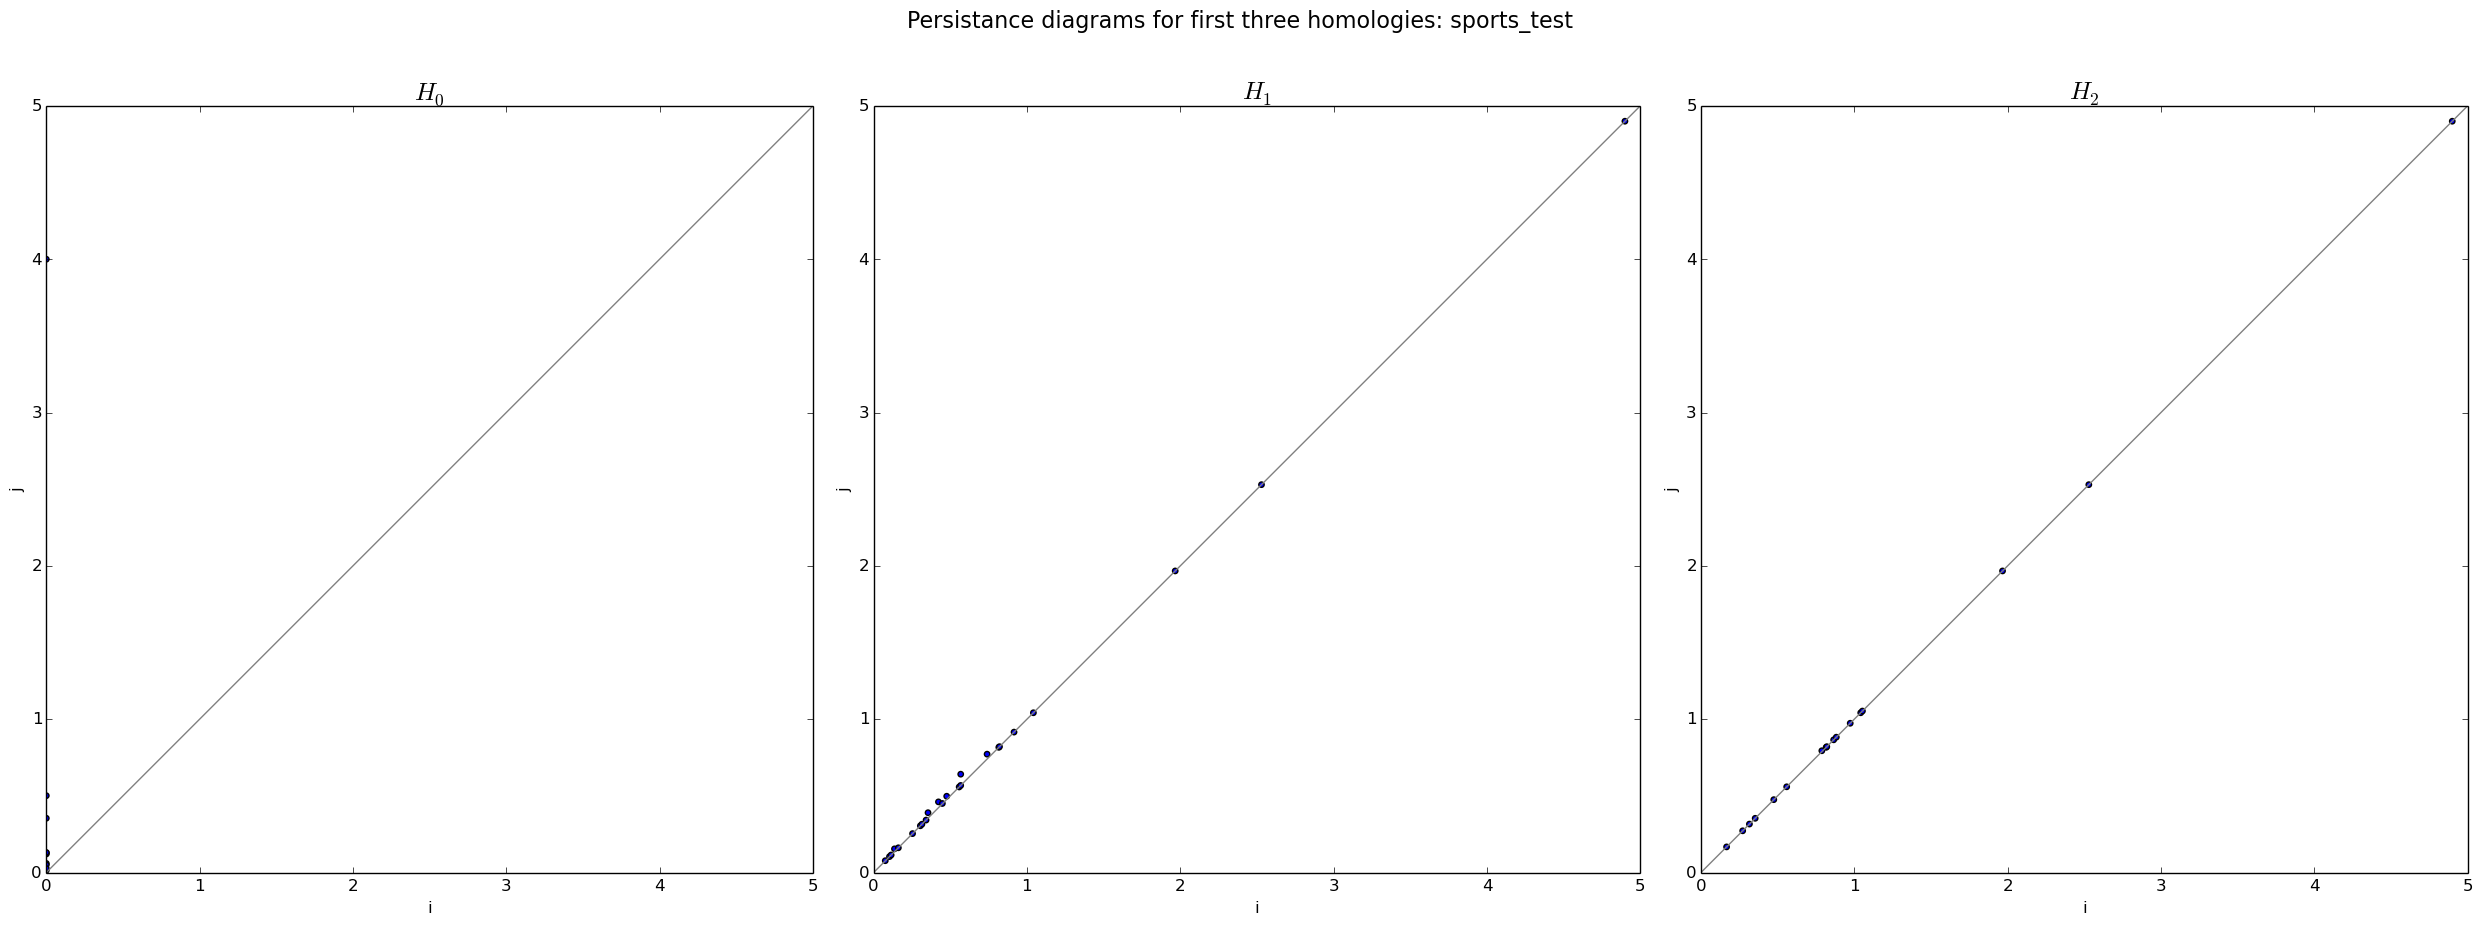
\includegraphics[width=\textwidth]{{img/pers_diagram_sports_test.png}}
  \caption{Persistance diagrams for sports\_test}
  \label{fig:s_4}
\end{figure}

%*********%
% reviews %
%*********%

\begin{figure}[H]
  \centering
  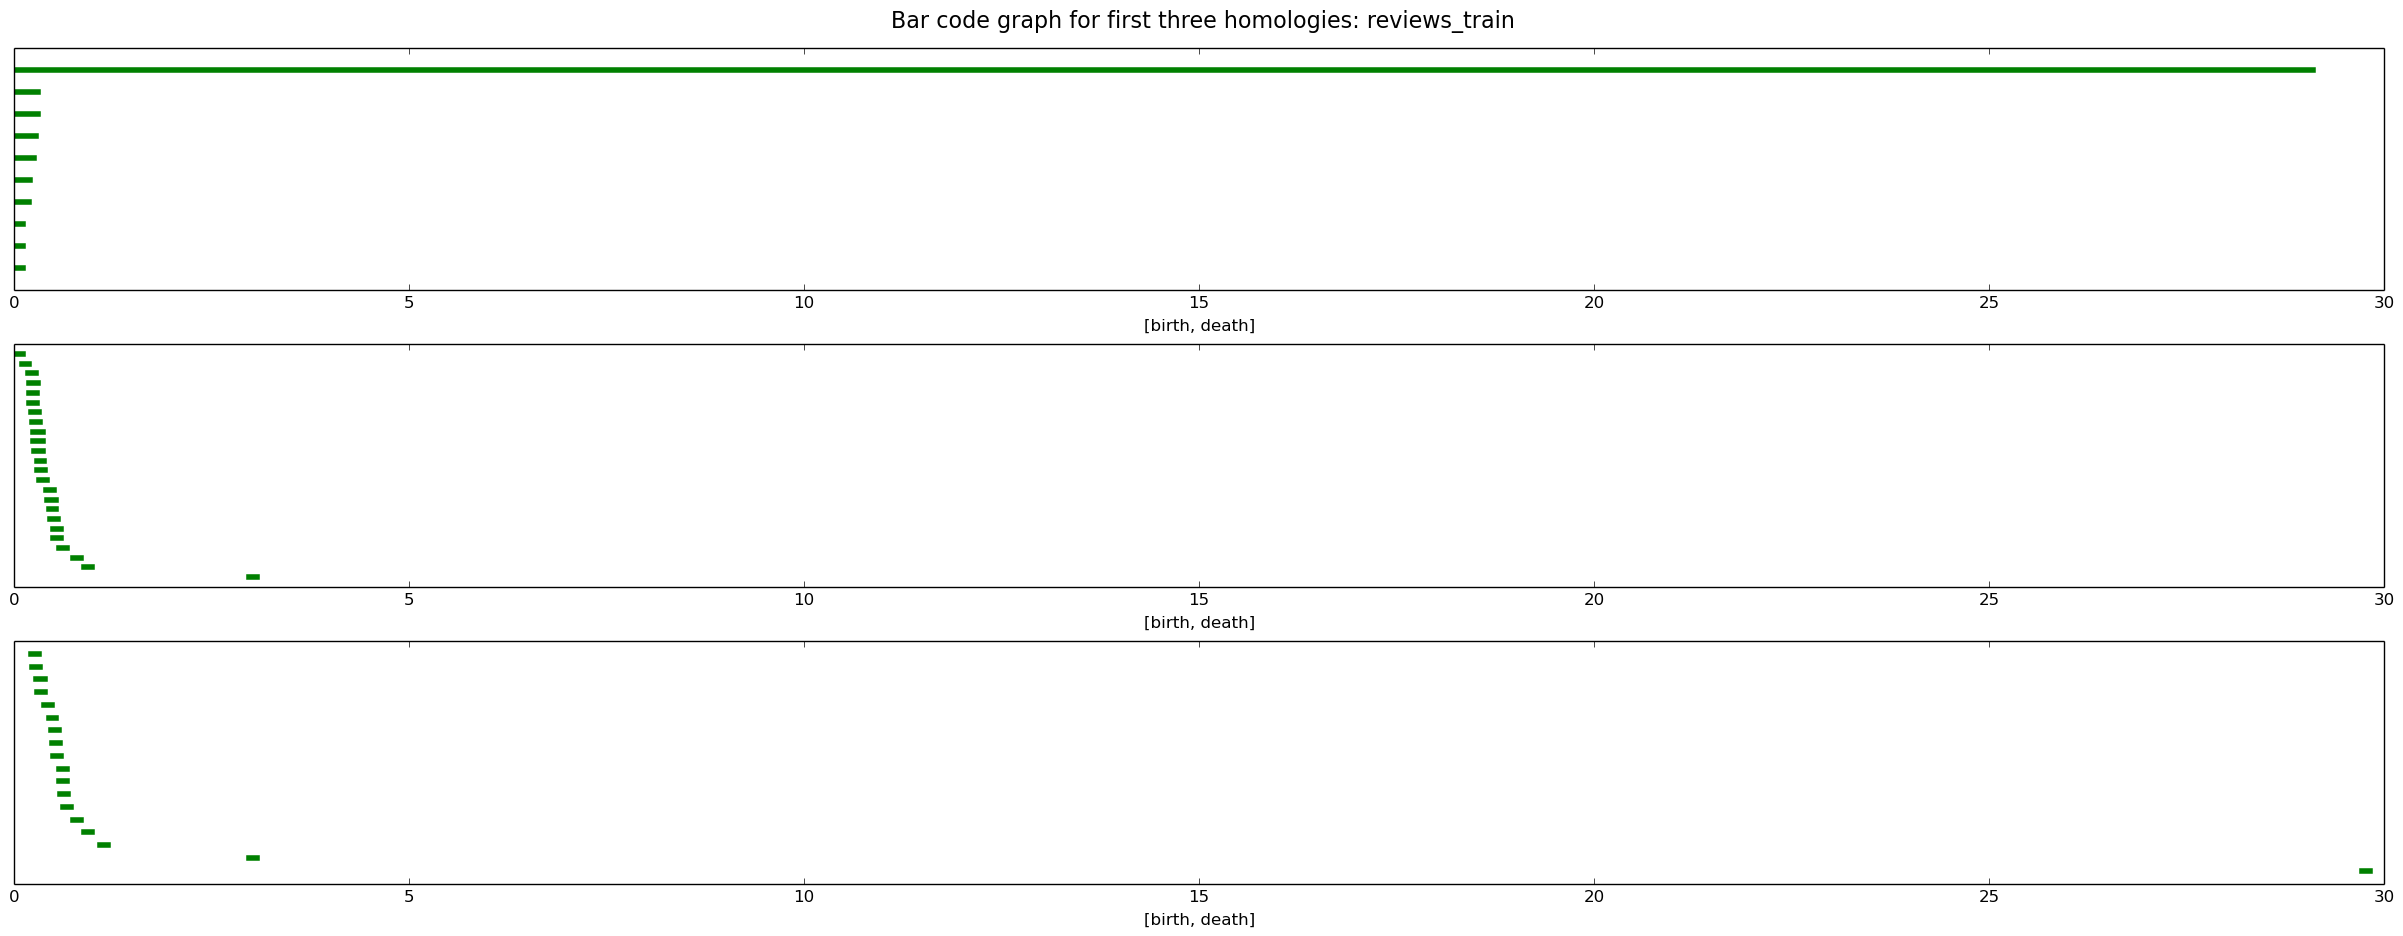
\includegraphics[width=\textwidth]{{img/bar_code_diagram_reviews_train.png}}
  \caption{Bar codes for reviews\_train}
  \label{fig:s_1}
\end{figure}
    
\begin{figure}[H]
  \centering
  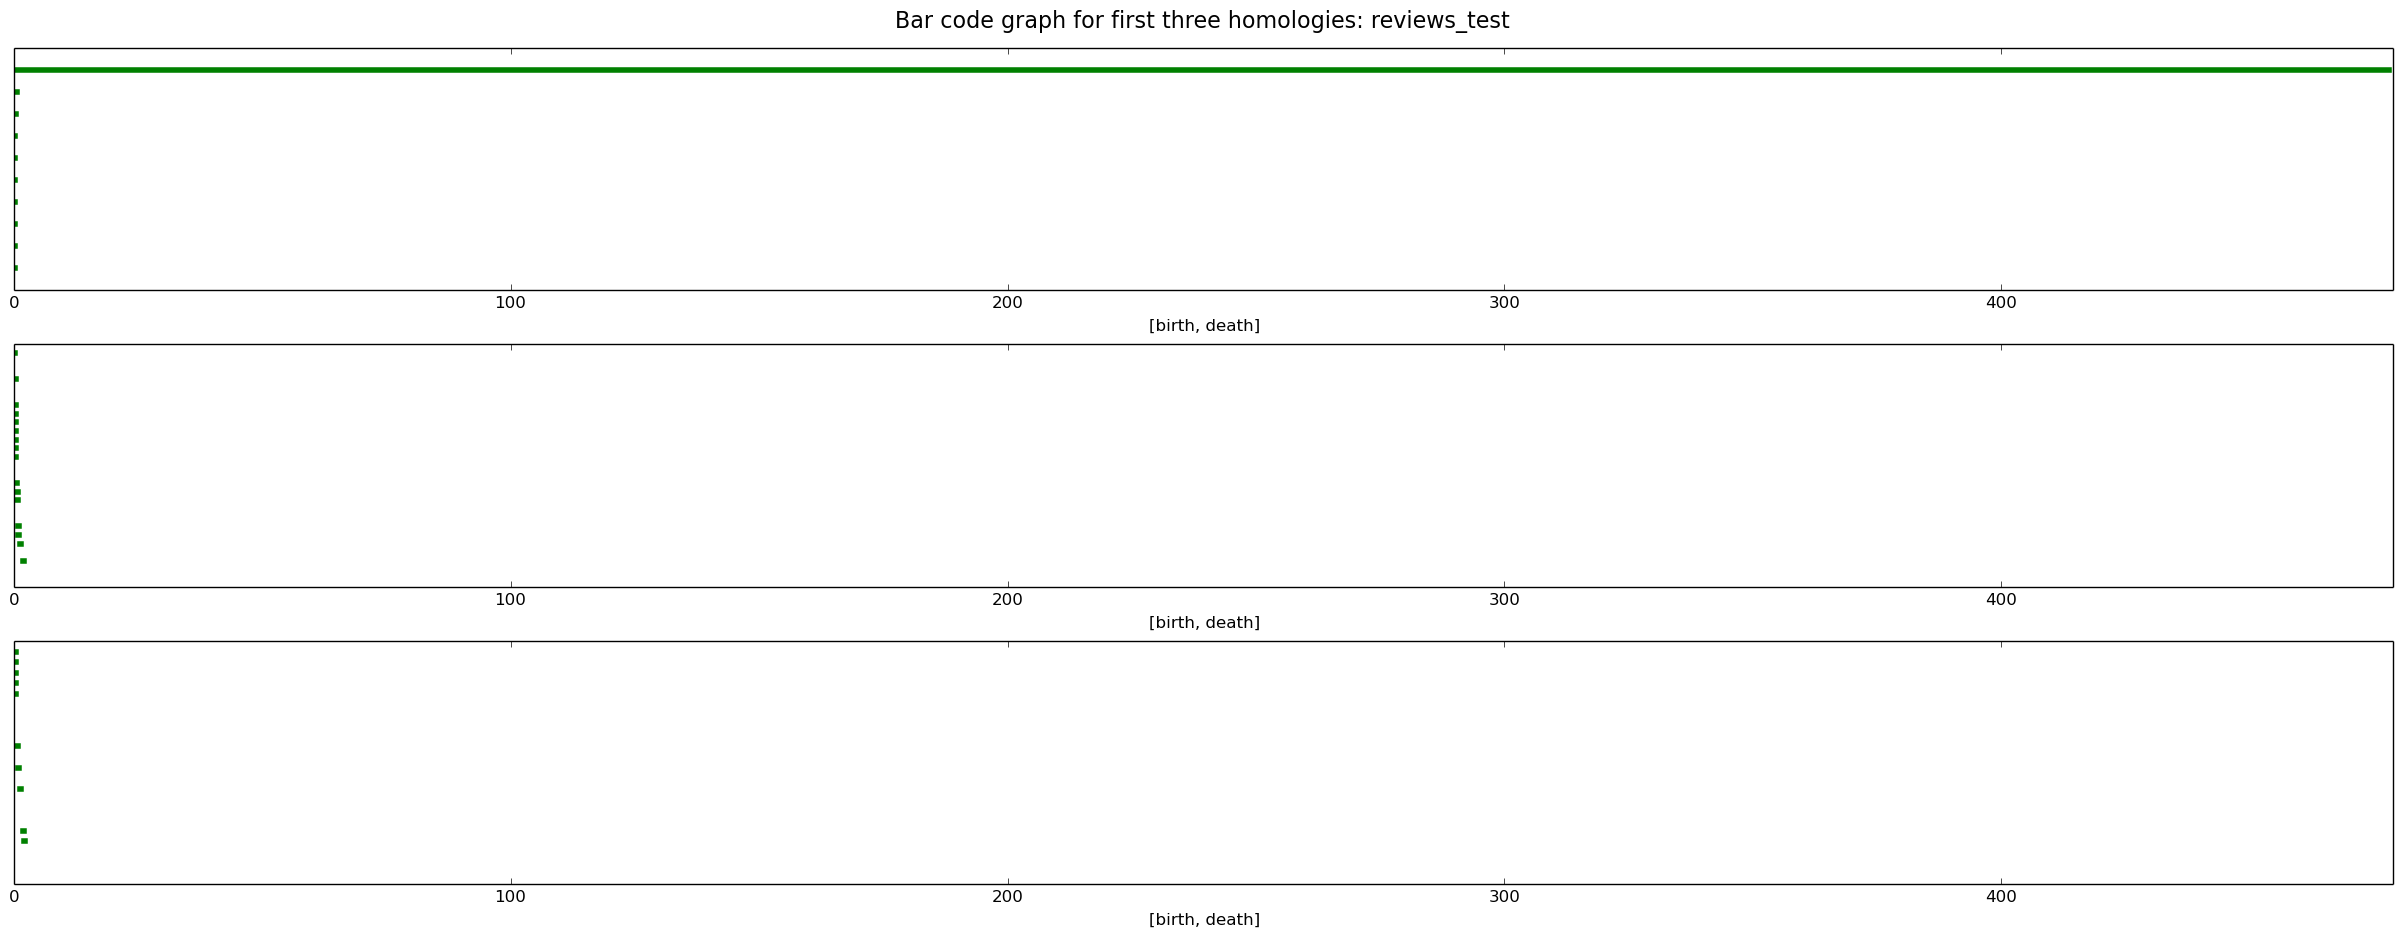
\includegraphics[width=\textwidth]{{img/bar_code_diagram_reviews_test.png}}
  \caption{Bar codes for reviews\_test}
  \label{fig:s_2}
\end{figure}

\begin{figure}[H]
  \centering
  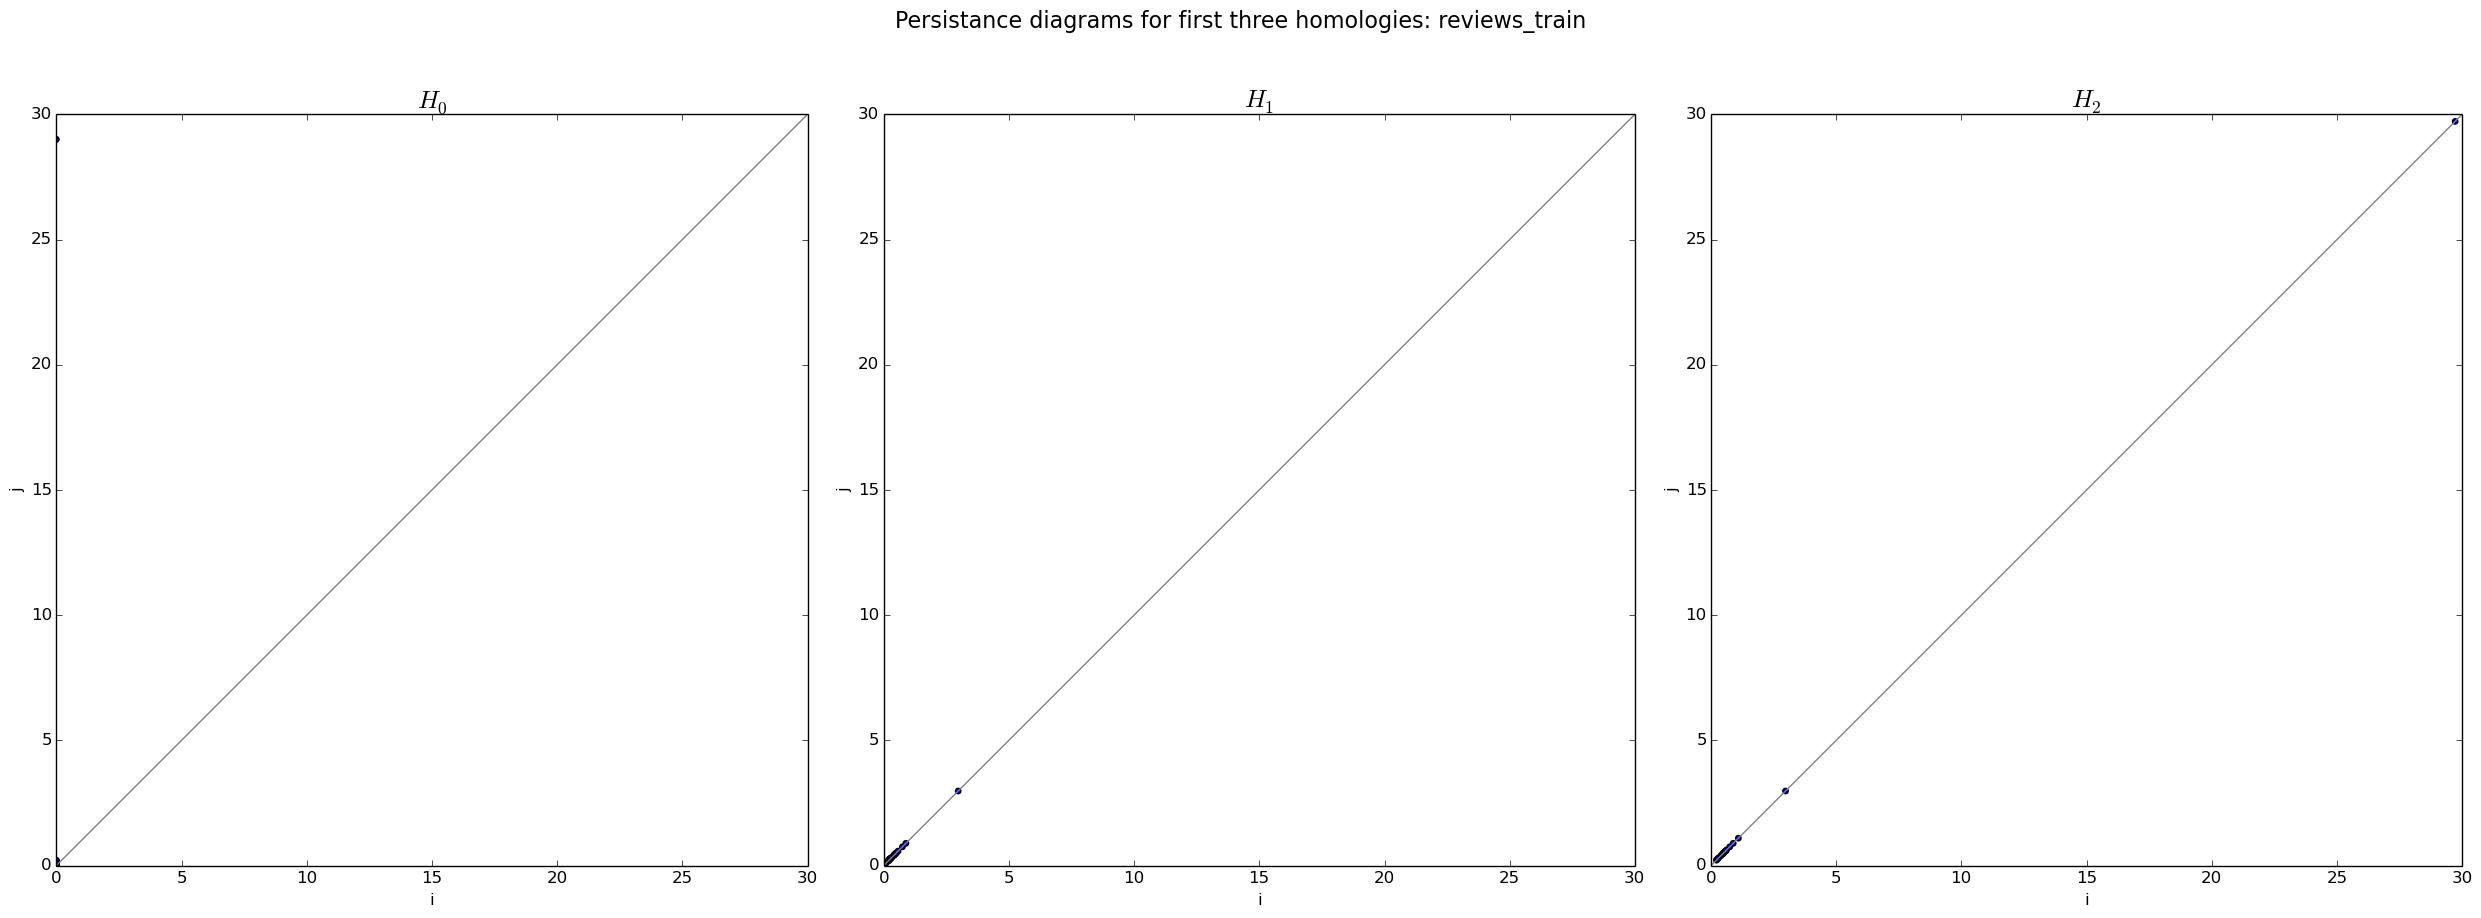
\includegraphics[width=\textwidth]{{img/pers_diagram_reviews_train.png}}
  \caption{Persistance diagrams for reviews\_train}
  \label{fig:s_3}
\end{figure}

\begin{figure}[H]
  \centering
  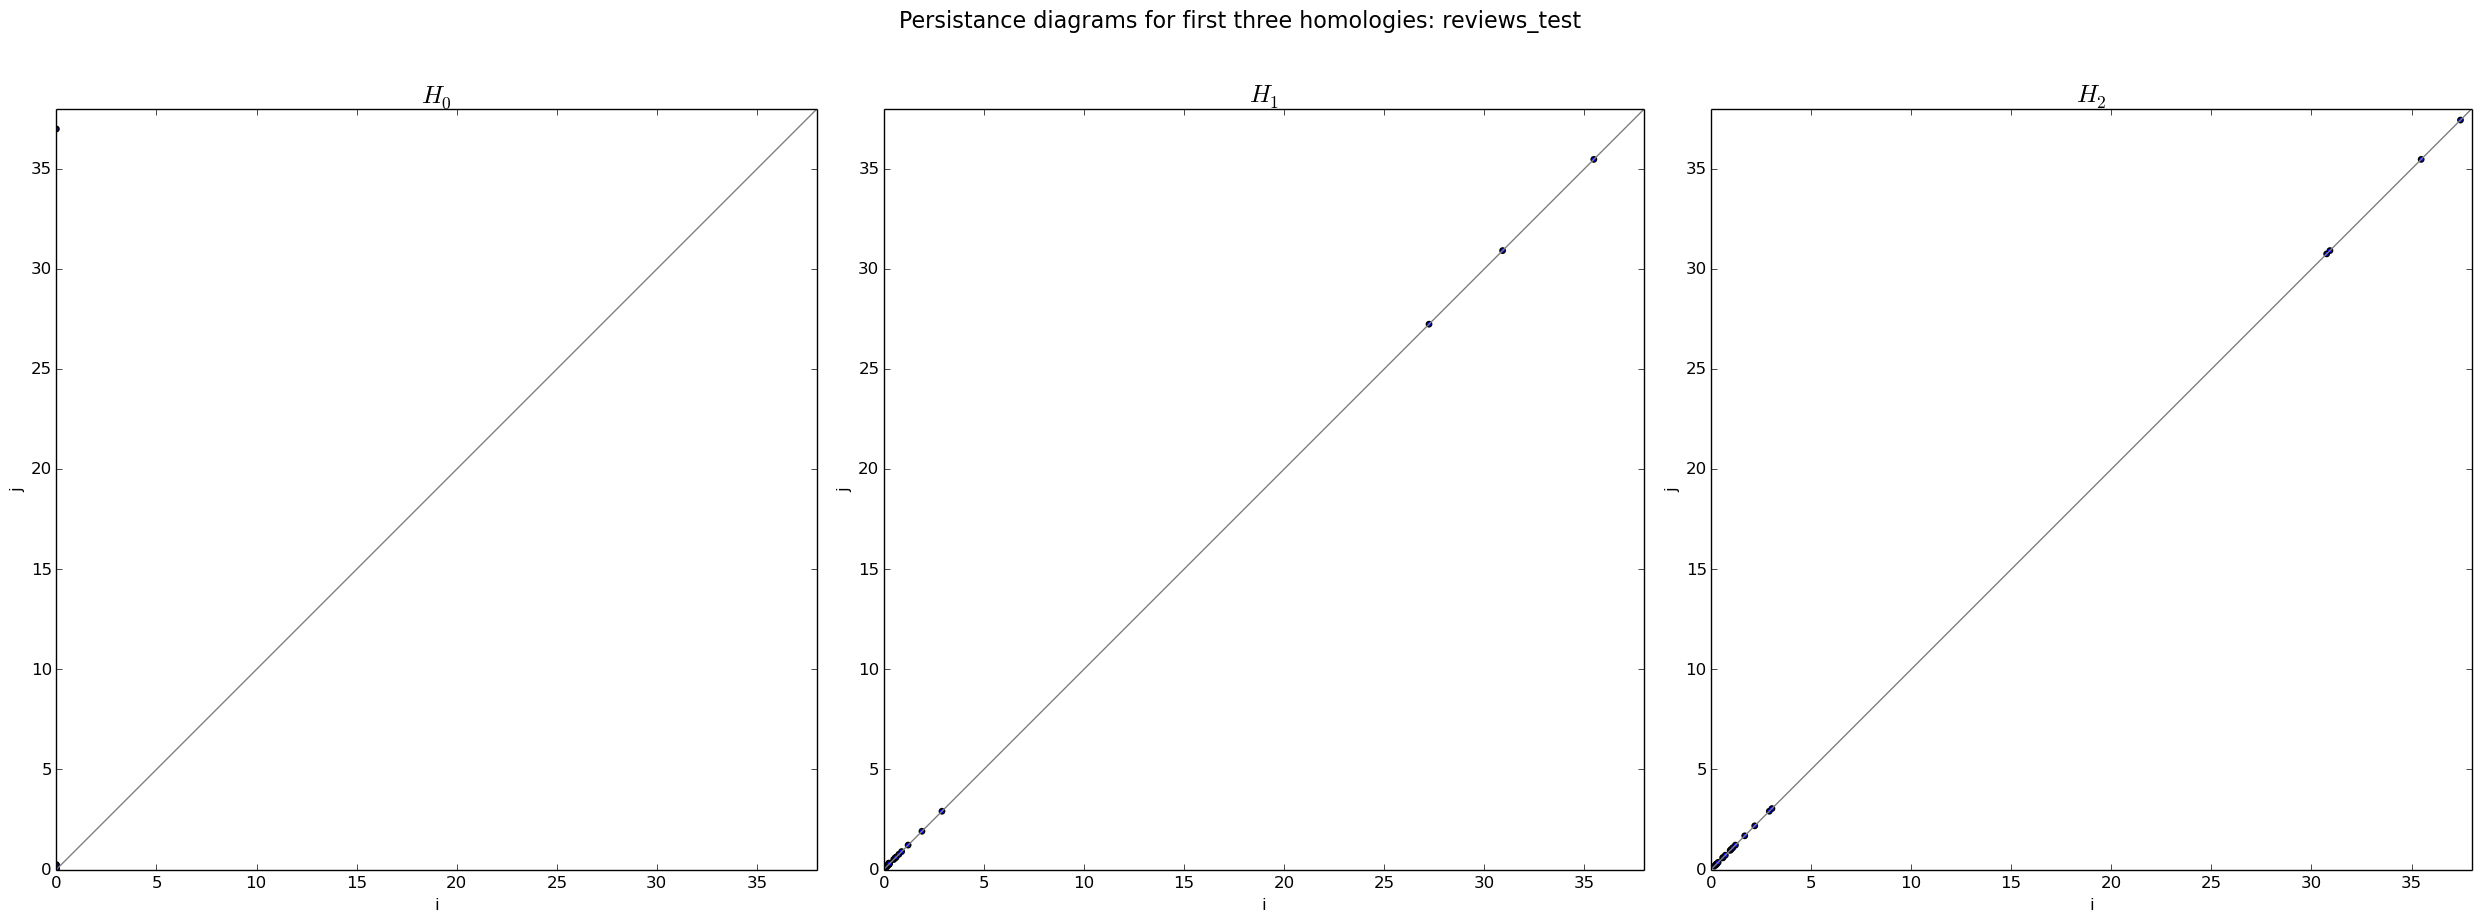
\includegraphics[width=\textwidth]{{img/pers_diagram_reviews_test.png}}
  \caption{Persistance diagrams for reviews\_test}
  \label{fig:s_4}
\end{figure}
